% Options for packages loaded elsewhere
\PassOptionsToPackage{unicode}{hyperref}
\PassOptionsToPackage{hyphens}{url}
%
\documentclass[
]{article}
\usepackage{lmodern}
\usepackage{amssymb,amsmath}
\usepackage{ifxetex,ifluatex}
\ifnum 0\ifxetex 1\fi\ifluatex 1\fi=0 % if pdftex
  \usepackage[T1]{fontenc}
  \usepackage[utf8]{inputenc}
  \usepackage{textcomp} % provide euro and other symbols
\else % if luatex or xetex
  \usepackage{unicode-math}
  \defaultfontfeatures{Scale=MatchLowercase}
  \defaultfontfeatures[\rmfamily]{Ligatures=TeX,Scale=1}
\fi
% Use upquote if available, for straight quotes in verbatim environments
\IfFileExists{upquote.sty}{\usepackage{upquote}}{}
\IfFileExists{microtype.sty}{% use microtype if available
  \usepackage[]{microtype}
  \UseMicrotypeSet[protrusion]{basicmath} % disable protrusion for tt fonts
}{}
\makeatletter
\@ifundefined{KOMAClassName}{% if non-KOMA class
  \IfFileExists{parskip.sty}{%
    \usepackage{parskip}
  }{% else
    \setlength{\parindent}{0pt}
    \setlength{\parskip}{6pt plus 2pt minus 1pt}}
}{% if KOMA class
  \KOMAoptions{parskip=half}}
\makeatother
\usepackage{xcolor}
\IfFileExists{xurl.sty}{\usepackage{xurl}}{} % add URL line breaks if available
\IfFileExists{bookmark.sty}{\usepackage{bookmark}}{\usepackage{hyperref}}
\hypersetup{
  pdftitle={Accounting for seed rain and other confounders reveals which ecosystems are most susceptible to alien conifer establishment},
  pdfauthor={Julien Vollering; Siri Lie Olsen; Olav Skarpaas; Leif Appelgren; Magni Olsen Kyrkjeeide; Anders Often; Jakob Sandven; Odd Stabbetorp; Øyvind Sørhuus},
  hidelinks,
  pdfcreator={LaTeX via pandoc}}
\urlstyle{same} % disable monospaced font for URLs
\usepackage{longtable,booktabs}
% Correct order of tables after \paragraph or \subparagraph
\usepackage{etoolbox}
\makeatletter
\patchcmd\longtable{\par}{\if@noskipsec\mbox{}\fi\par}{}{}
\makeatother
% Allow footnotes in longtable head/foot
\IfFileExists{footnotehyper.sty}{\usepackage{footnotehyper}}{\usepackage{footnote}}
\makesavenoteenv{longtable}
\usepackage{graphicx,grffile}
\makeatletter
\def\maxwidth{\ifdim\Gin@nat@width>\linewidth\linewidth\else\Gin@nat@width\fi}
\def\maxheight{\ifdim\Gin@nat@height>\textheight\textheight\else\Gin@nat@height\fi}
\makeatother
% Scale images if necessary, so that they will not overflow the page
% margins by default, and it is still possible to overwrite the defaults
% using explicit options in \includegraphics[width, height, ...]{}
\setkeys{Gin}{width=\maxwidth,height=\maxheight,keepaspectratio}
% Set default figure placement to htbp
\makeatletter
\def\fps@figure{htbp}
\makeatother
\setlength{\emergencystretch}{3em} % prevent overfull lines
\providecommand{\tightlist}{%
  \setlength{\itemsep}{0pt}\setlength{\parskip}{0pt}}
\setcounter{secnumdepth}{5}
\usepackage{pdflscape}
\newcommand{\blandscape}{\begin{landscape}}
\newcommand{\elandscape}{\end{landscape}}
\usepackage{booktabs}
\usepackage{longtable}
\usepackage{array}
\usepackage{multirow}
\usepackage{wrapfig}
\usepackage{float}
\usepackage{colortbl}
\usepackage{pdflscape}
\usepackage{tabu}
\usepackage{threeparttable}
\usepackage{threeparttablex}
\usepackage[normalem]{ulem}
\usepackage{makecell}
\usepackage{xcolor}

\title{Accounting for seed rain and other confounders reveals which ecosystems are most susceptible to alien conifer establishment}
\author{Julien Vollering\footnote{\href{mailto:julienvollering@gmail.com}{\nolinkurl{julienvollering@gmail.com}}} \and Siri Lie Olsen \and Olav Skarpaas \and Leif Appelgren \and Magni Olsen Kyrkjeeide \and Anders Often \and Jakob Sandven \and Odd Stabbetorp \and Øyvind Sørhuus}
\date{}

\begin{document}
\maketitle

{
\setcounter{tocdepth}{2}
\tableofcontents
}
\hypertarget{orcids}{%
\section{ORCIDs}\label{orcids}}

Julien Vollering: \url{https://orcid.org/0000-0002-7409-2898}

Siri Lie Olsen: \url{https://orcid.org/0000-0002-4443-8261}

Olav Skarpaas: \url{https://orcid.org/0000-0001-9727-1672}

Magni Olsen Kyrkjeeide: \url{https://orcid.org/0000-0002-7454-3652}

\hypertarget{abstract}{%
\section{Abstract}\label{abstract}}

\begin{enumerate}
\def\labelenumi{\arabic{enumi}.}
\tightlist
\item
  Plantations of alien conifer species are common worldwide, and set to become even more prevalent in coming decades. The rate at which their offspring colonize surroundings varies among plantations, and the reasons for this variation are often unclear. To minimize the spread of so-called ``wildlings'' and the burden of conifer plantations on native ecosystems, managers need to know which ecosystems are most and least susceptible.
\item
  We compared how likely wildlings are to establish across a wide range of ecosystems, focusing on four groups of alien conifer species planted in Norway. We used data from detailed surveys around 82 plantations to model the relationship between ecosystem type and wildling abundance --- accounting for seed rain, climate, and other sources of variation between sites. Furthermore, we tested whether differences in susceptibility between individual ecosystem types could be generalized based on broad, shared characteristics.
\item
  We found that the rank order of ecosystems by susceptibility (modeled as relative establishment likelihood) differed from their rank order by wildling density. Moreover, ecosystem susceptibility tended to vary more than wildling density. For all species groups, relative establishment likelihoods spanned several orders of magnitude between the most and least susceptible ecosystems.
\item
  The four groups of conifer species showed somewhat similar patterns of establishment likelihood across ecosystem types, with intensively farmed ecosystems repeatedly among the least susceptible. We found that ecosystems characterized by destabilizing disturbance tended to be most susceptible, but broad ecosystem characteristics did not clarify patterns of susceptibility much, neither within nor across species groups.
\item
  \emph{Synthesis and applications} Differences in wildling establishment between ecosystems can be exploited to keep alien conifers within plantation boundaries. Plantations hemmed in by agriculture or other unsusceptible ecosystems will result in relatively few wildlings, while plantations near landslides and other susceptible ecosystems will need monitoring and control. Managers should be aware that the density of wildlings in a given ecosystem may not reflect its relative susceptibility, because variation in seed rain, climate, and site characteristics obscures the relationship between ecosystem type and wildling establishment.
\end{enumerate}

\hypertarget{keywords}{%
\section{Keywords}\label{keywords}}

alien species, conifer, establishment likelihood, disturbance, invasibility, plantation, recruitment, seed dispersal, Wald Analytical Long-distance Dispersal (WALD)

\hypertarget{introduction}{%
\section{Introduction}\label{introduction}}

Plantations of alien conifers are widespread globally, and offspring from these plantations frequently establish in surrounding areas (Richardson and Rejmánek \protect\hyperlink{ref-richardsonConifersInvasiveAliens2004}{2004}).
In many instances these naturalized offspring, or wildlings, harm biodiversity and other values, so controlling their spread is prudent.
In particular, plantations contribute to the presence of alien conifers in protected areas, and generate substantial control costs as a result (McConnachie et al. \protect\hyperlink{ref-mcconnachieEstimatingEffectPlantations2015}{2015}).
Controlling wildlings protects plantation surroundings and prevents secondary, potentially invasive spread.
Accordingly, guidelines for sustainable use of alien trees stress that containing them to the areas set aside for their cultivation is fundamental to good forestry practice (Brundu et al. \protect\hyperlink{ref-brunduGlobalGuidelinesSustainable2020}{2020}).

How many wildlings are present and how far they are from the plantation varies a lot from site to site, even among conspecific plantations of similar age (Nygaard and Øyen \protect\hyperlink{ref-nygaardSpreadIntroducedSitka2017}{2017}, Fernandes et al. \protect\hyperlink{ref-fernandesWhatDrivesEucalyptus2018}{2018}), which makes it harder to predict and manage their spread.
To begin to understand this variation, we need to consider both dispersal and establishment (where establishment comprises germination and survival).
These jointly generate patterns of wildling abundance and spatial distribution.
Dispersal at a given site is affected by conditions related to a species' dispersal syndrome --- for instance wind exposure and site topography, in the case of a wind-dispersed species.
Likewise, establishment is affected by biotic and abiotic conditions where seeds arrive.
In theory, conditions inhibiting either process may be exploited to suppress wildling spread.

Reducing establishment is of particular interest because it directly regulates wildling abundance.
The conditions affecting establishment are also generally easier to manipulate than those affecting dispersal, either directly through intervention or indirectly through site selection.
The question, then, becomes: how can we identify establishment-inhibiting conditions in a manner applicable to plantation management?

In Norway --- and similarly in other countries --- the national land mapping classification system sorts variation in local ecological conditions (Halvorsen et al. \protect\hyperlink{ref-halvorsenSystematicsEcodiversityEcoSyst2020}{2020}).
It builds on the continuum concept (Austin \protect\hyperlink{ref-austinContinuumConceptOrdination1985}{1985}), aiming for reproducible and value-neutral classification of ecosystems by rule-based discretization of species turnover along important environmental gradients (Halvorsen et al. \protect\hyperlink{ref-halvorsenSystematicsEcodiversityEcoSyst2020}{2020}).
As a result, it encapsulates in its ecosystem types (hereafter: ``ecosystems'') much of the variation that is most likely to regulate wildling germination and survival --- in competition, nutrient availability, disturbance, and the like (Richardson and Pyšek \protect\hyperlink{ref-richardsonNaturalizationIntroducedPlants2012}{2012}).
It also identifies broad similarities between ecosystems, which might be used to tease out generic trends in establishment likelihood.

To estimate how likely wildlings are to establish in particular ecosystems based on observations of their abundance around plantations, we must account for (1) seed dispersal, and (2) sources of variation in establishment beside ecosystem type.
For example, low establishment likelihood in an ecosystem frequently located close to plantations can be masked by copious seed rain (Rouget and Richardson \protect\hyperlink{ref-rougetInferringProcessPattern2003}{2003}).
Likewise, an ecosystem may appear to promote establishment if it tends to co-occur with climatic conditions that support germination.
Unconfounded establishment likelihoods can then be used to predict how susceptible the surroundings of an unobserved plantation are, based on its composition of ecosystems.

Determining which ecosystems are most susceptible so that interventions can be prioritized objectively is among the most urgent objectives for invasion science (Pyšek et al. \protect\hyperlink{ref-pysekScientistsWarningInvasive2020}{2020}).
Plantations of wind-dispersed, alien conifers present an opportunity to assess ecosystem invasibility (to these species), because we can estimate ecosystem exposure (seed rain) directly, rather than by proxy (Catford et al. \protect\hyperlink{ref-catfordQuantifyingLevelsBiological2012}{2012}).
We examine plantations of alien conifers in Norway to investigate the following questions:

\begin{enumerate}
\def\labelenumi{\arabic{enumi}.}
\tightlist
\item
  How do estimates of establishment likelihood differ from observed wildling densities?
\item
  In which ecosystems are wildlings of alien conifers most and least likely to establish?
\item
  Can overarching characteristics of ecosystems be used to generalize patterns of wildling establishment?
\end{enumerate}

\hypertarget{methods}{%
\section{Methods}\label{methods}}

\hypertarget{field-data}{%
\subsection{Field data}\label{field-data}}

We registered wildlings and ecosystems around 82 plantations across Norway, comprising four groups of alien conifers (hereafter: ``species''; fig.~\ref{fig:sites-map}).
The sample contained (1) forty-two sites with Sitka spruce (\emph{Picea sitchensis}) or its fertile hybrid, Lutz spruce (\emph{Picea} x \emph{lutzii}), (2) nineteen with Norway spruce (\emph{Picea abies}), (3) fifteen with larch species (\emph{Larix} spp.), and (4) six with lodgepole pine (\emph{Pinus contorta}).
Note that Norway spruce is native to Norway, but the plantations included in this study were located in parts of the country where its natural distribution is highly restricted.
We selected and delineated plantations manually --- using aerial imagery --- aiming for plantations that were isolated from other plantations of the same species.
Only plantations with cone-bearing individuals were included in the sample.
We collected field data from each plantation in one of six field campaigns during the period 2016-2019 (reported in Olsen et al. \protect\hyperlink{ref-olsenKartleggingAvKortdistansespredning2016}{2016}, \protect\hyperlink{ref-olsenKartleggingAvKortdistansespredning2019}{2019}, Appelgren and Torvik \protect\hyperlink{ref-appelgrenKartleggingAvKortdistansespredning2017}{2017}, Kyrkjeeide et al. \protect\hyperlink{ref-kyrkjeeideKartleggingAvKortdistansespredning2017}{2017}, Appelgren \protect\hyperlink{ref-appelgrenKartleggingAvKortdistansespredning2018}{2018}, Sandven et al. \protect\hyperlink{ref-sandvenKartleggingAvKortdistansespredning2019}{2019}).

\begin{figure}
\centering
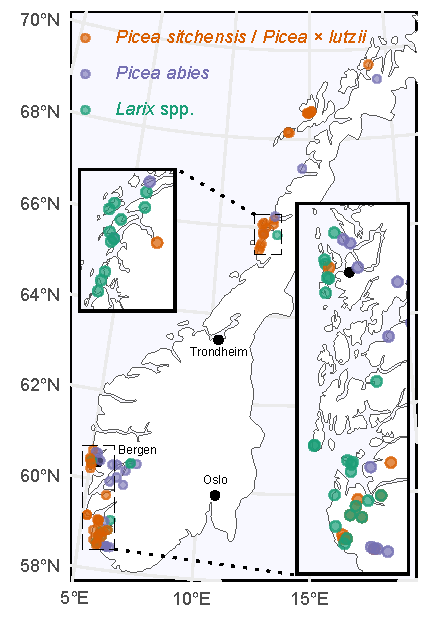
\includegraphics{figures/sites-map.pdf}
\caption{\label{fig:sites-map}Locations of the 82 plantations in the data set.}
\end{figure}

In the field, wildlings and ecosystems were mapped comprehensively within a 500x500 m plot framing the plantation of interest.
Except in the 2016 field campaign, we also mapped as polygons any additional plantations of the same species within a larger 2x2 km plot.
We used GPS to register the point-positions of all wildlings over 30 cm in height, recording a single position for groups of wildlings occurring with less than 5 m between them.
A few exceptionally dense groups of wildlings were mapped by registering polygons instead of points and estimating the number of individuals by transect counts.
Concurrently, we registered polygons for all terrestrial ecosystems, following the Nature in Norway classification system (version 2.0 or 2.1, Halvorsen et al. \protect\hyperlink{ref-halvorsenNaturNorgeNiN2015}{2015}, based on the principles summarized in \protect\hyperlink{ref-halvorsenSystematicsEcodiversityEcoSyst2020}{2020}).
The Nature in Norway system is the national standard for land cover mapping and provides full spatial coverage (i.e.~any location and any kind of land cover is assignable to an ecosystem).
We mapped ecosystems at a scale of 1:5000, which implies that all polygons with a size over 250 m\textsuperscript{2} were registered (Bryn and Halvorsen \protect\hyperlink{ref-brynVeilederKartleggingAv2015}{2015}).
Regularly patterned occurrence of more than one ecosystem in polygons smaller than the minimum size were registered as so-called mosaic polygons.

For each of the central plantations we measured the height of a representative individual in the plantation by clinometer.
We also estimated the age of the plantation at the time of the field campaign, either by contacting land owners or municipal officials, or by counting growth rings.
Details for all 82 plantations are provided in the Appendix (table \ref{tab:sites-table}).

\hypertarget{seed-dispersal}{%
\subsection{Seed dispersal}\label{seed-dispersal}}

To account for the influence of seed dispersal on wildling abundance, we needed estimates of the spatial distribution of seed rain within the 500x500 m field plots.
Conspecific plantations were sometimes located nearby the central plantation, so we considered all plantations within a 1 km radius to be potential seed sources.
We used two models of seed dispersal to derive two different estimates of relative seed rain in space.
Acknowledging the uncertainty involved in estimating seed dispersal (Nathan et al. \protect\hyperlink{ref-nathanDispersalKernels2012}{2012}), we explored one empirically-parameterized, isotropic model and one mechanistically-derived, anisotropic model.

The first model was a static seed dispersal kernel with parameter estimates generalized from multiple data sets.
Specifically, we selected from Bullock et al.~(\protect\hyperlink{ref-bullockSynthesisEmpiricalPlant2017}{2017}) the kernel that performed best for wind-adapted seeds from 5-15 m tall trees (an Exponential Power function).
Seventy-two of the 82 plantations in our data set matched this height range better than a taller range with a different empirical kernel.

The second model was an anisotropic implementation of the Wald Analytical Long-distance Dispersal (WALD, Katul et al. \protect\hyperlink{ref-katulMechanisticAnalyticalModels2005}{2005}) model, following Skarpaas \& Shea (\protect\hyperlink{ref-skarpaasDispersalPatternsDispersal2007}{2007}).
We parameterized the model with: site- and season-specific wind vectors retrieved from meteorological data sets, wind turbulence estimated from local ecosystem composition, seed release height based on plantation height, and species-specific seed terminal velocities from literature.

We transformed field-mapped polygons of seed sources into hexagonally gridded point sources, with a density of 0.1 m\textsuperscript{-2} for the first model and 0.01 m\textsuperscript{-2} for the second model (to reduce computation time).
Then we applied our two dispersal models to estimate the distribution of relative seed rain from all point sources in a grid of 10 m cells.
We chose this cell size to be similar to the smallest allowed ecosystem polygon.

A full description of our implementation of the WALD model and additional details about seed source polygons are given in the \protect\hyperlink{appendix}{Appendix}.

\hypertarget{establishment-likelihood}{%
\subsection{Establishment likelihood}\label{establishment-likelihood}}

For our analysis of establishment likelihood, we rasterized wildling occurrences and ecosystems to the same 10 m grid as the seed dispersal models (fig.~\ref{fig:site-example}).
Rather than assigning a single ecosystem to each grid cell, we applied fuzzy logic and assigned ecosystems in proportion to their areal coverage of the cell.
In other words, each ecosystem was rendered as a separate raster variable with values in the range {[}0,1{]}.
We allowed mixed cell composition to capture ecotones in the model and to try to avoid overreliance on the precision of mapped ecosystem boundaries.
Area covered by mosaic polygons was divided evenly among the constituent ecosystem types.
We excluded the ``tree plantation'' ecosystem from our analyses because some of the field campaigns did not register wildlings occurring there.
Grid cells comprised mostly of ``tree plantation'' (\textgreater{} 0.5) were dropped.
The resulting data set was used both to calculate densities of wildlings (abundance/area) and model relative establishment likelihoods.
For the density calculation, wildling abundance was tallied in proportion to the ecosystem composition of the grid cells they occupied.
For example, a cell occupied by three wildlings and half-covered by a given ecosystem would tally 1.5 wildlings for that ecosystem.

\begin{figure}
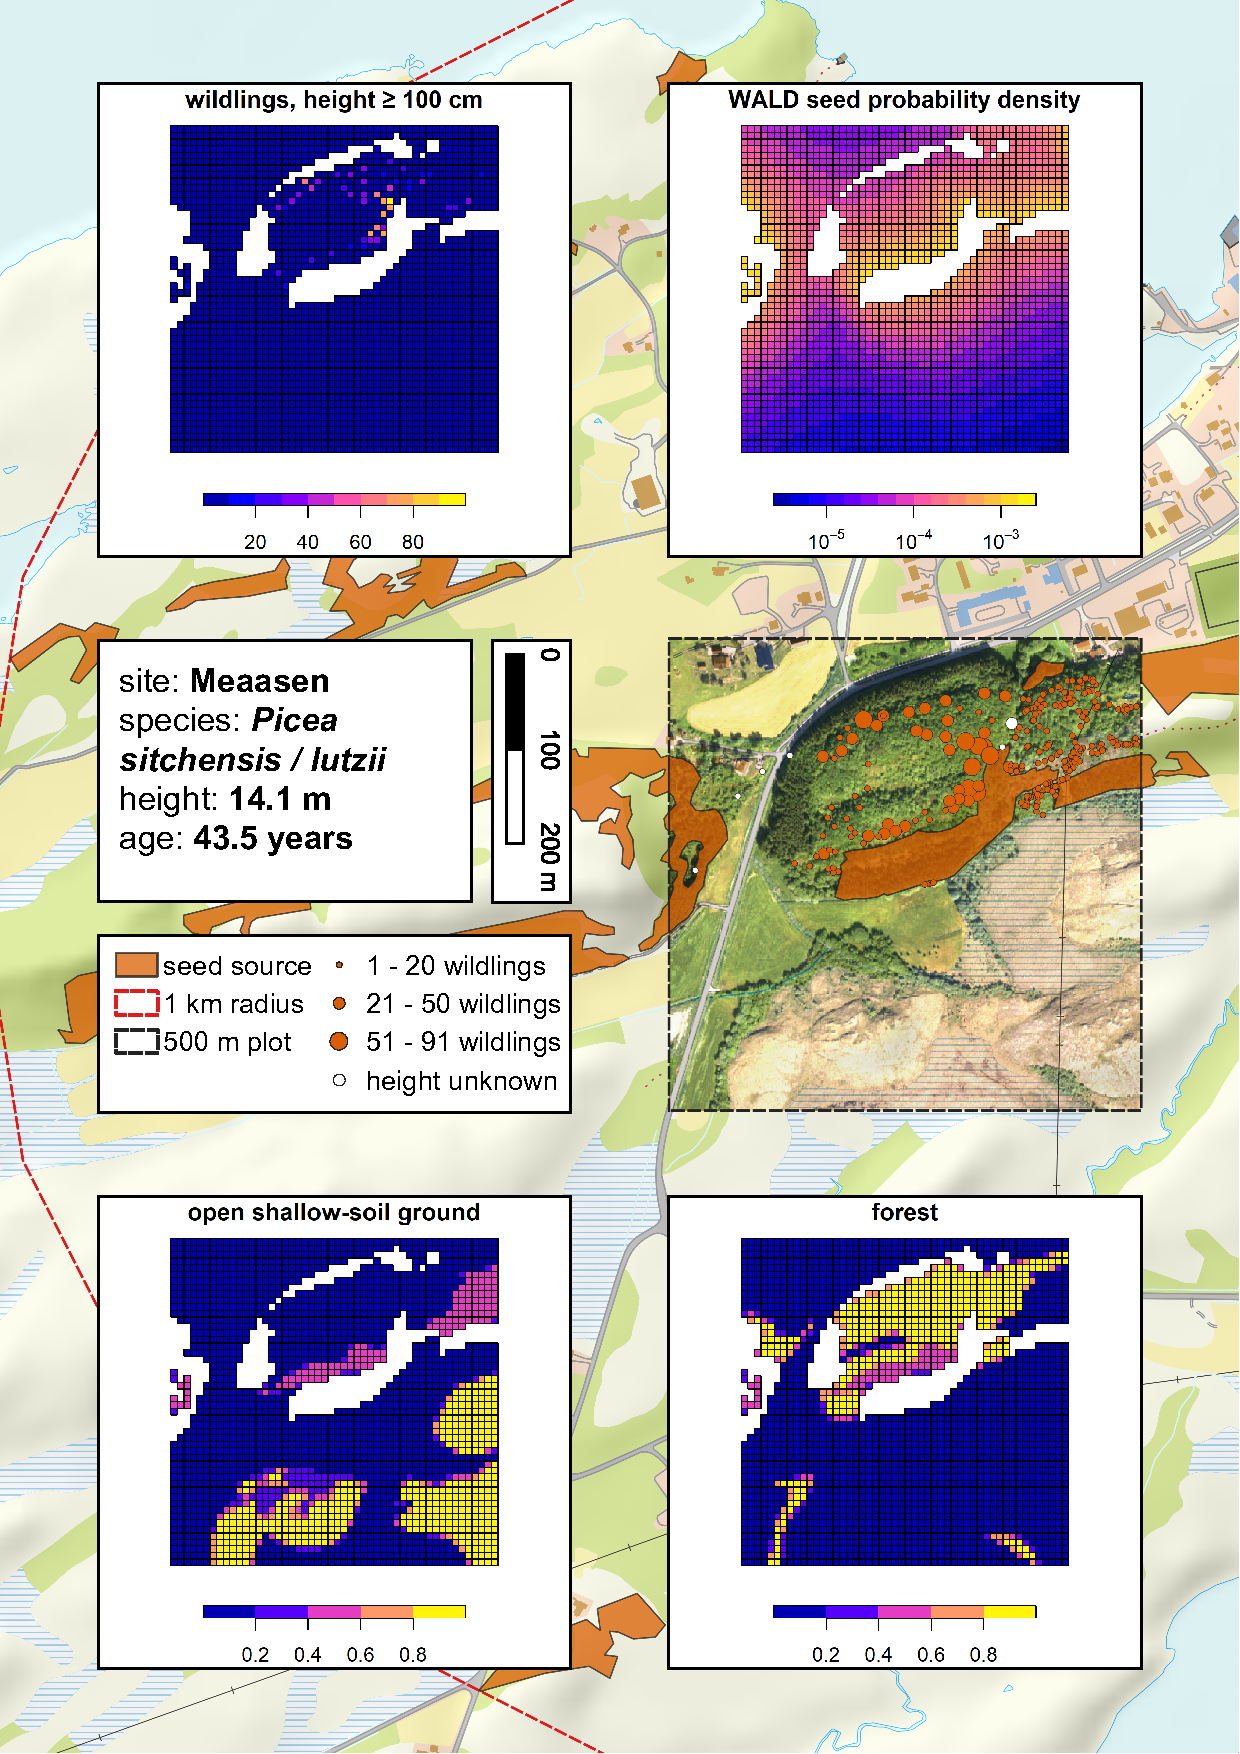
\includegraphics[width=0.9\linewidth]{figures/site-example/site-example} \caption{An illustration of one of the 82 plantation sites: Meaasen. The background map shows the surroundings of the plantation, and the 500x500 m plot is overlaid with an aerial photograph. The middle row of panels shows the data as registered in the field (but without ecosystem type polygons). The top and bottom rows of panels show selected variables for the 500x500 m plot, as used in the regression model (with a spatial grain of 10 m). Grid cells without data are either seed sources (corresponding to the polygons shown) or tree plantations of other species (such as one along the road).}\label{fig:site-example}
\end{figure}

We used a directed acyclic graph (DAG) to diagram causal relationships among the factors we expected to influence wildling abundance per cell (fig.~\ref{fig:DAG}).
In the DAG, the unmeasured, proximate causes of wildling abundance --- total seed rain over the lifetime of the plantation and establishment likelihood --- are descendants of variables that we could observe or model.
We included an effect of elevation from plantation on seed rain because neither of our models of seed dispersal account for uneven terrain.

\begin{figure}
\centering
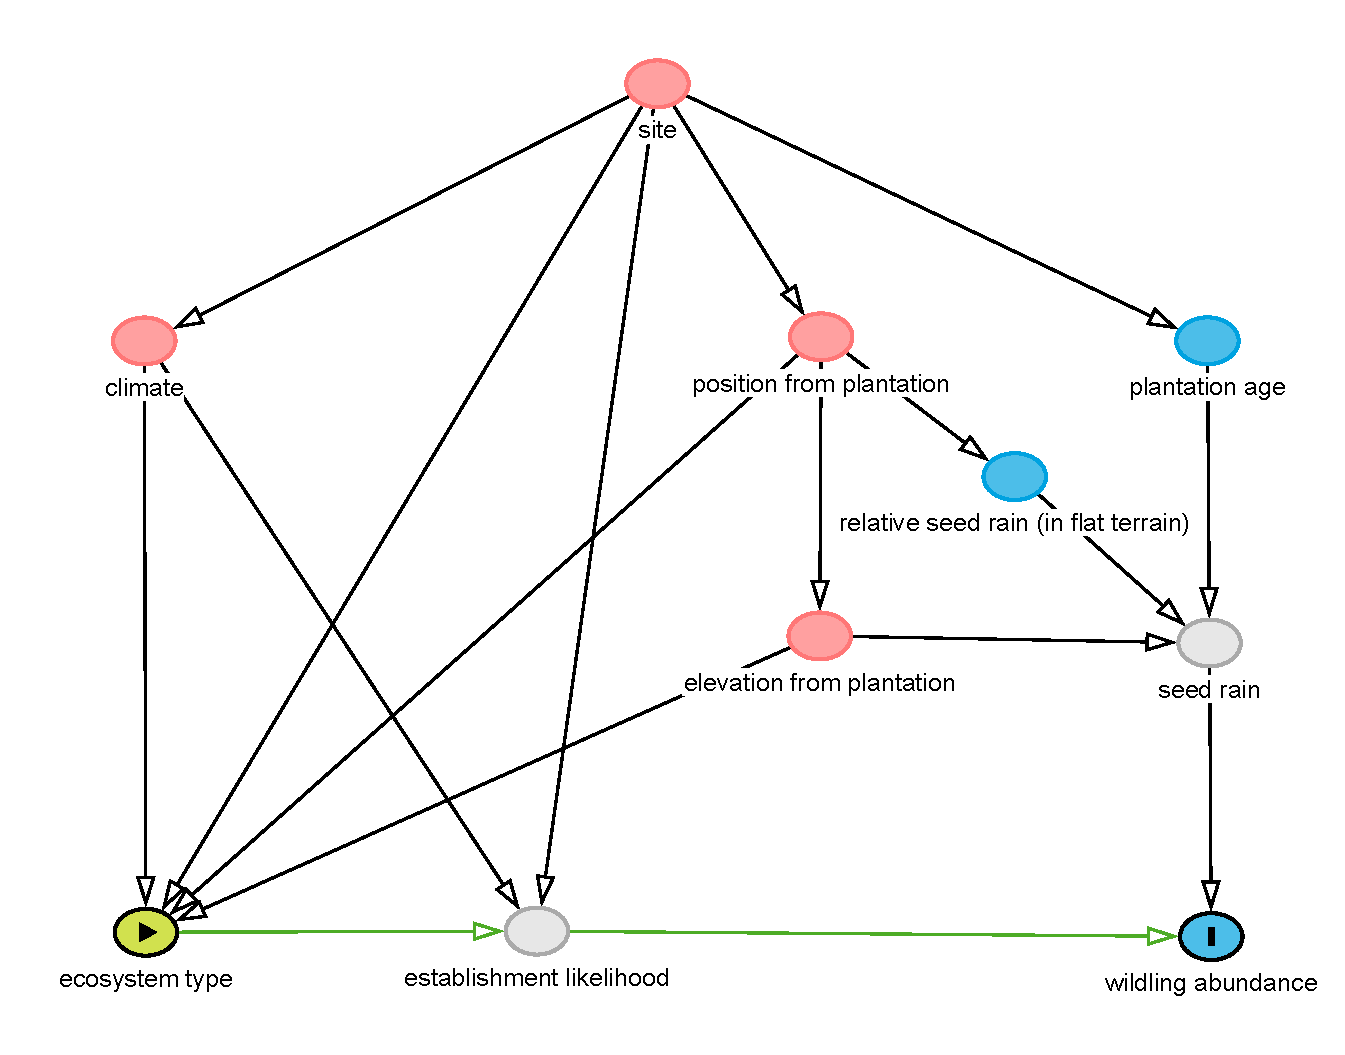
\includegraphics{/home/julien/Documents/dissertation/chapter3/conifer-plantation-spread/ms/figures/dagitty-model.pdf}
\caption{\label{fig:DAG}A directed acyclic graph showing the causal relationships motivating our statistical model of ecosystems' effects on wildling abundance. Red variables causally affect both the ecosystem type and wildling abundance, blue variables causally affect only wildling abundance, and grey variables are unobserved. Green arrows show the causal pathway of interest.}
\end{figure}

For all species, wildling abundance showed a high frequency of zeros that was underestimated by the best fitting negative binomial distribution.
Accordingly, we applied zero-inflated generalized linear models, fitted with the glmmTMB package (version 1.0, Brooks et al. \protect\hyperlink{ref-brooksGlmmTMBBalancesSpeed2017}{2017}) in R (version 3.6, R Core Team \protect\hyperlink{ref-rcoreteamLanguageEnvironmentStatistical2020}{2020}).
These zero-inflated models regard zeros as the mixed product of a binomial process as well as a (conditional) count process that can take different error distributions (Zuur et al. \protect\hyperlink{ref-zuurMixedEffectsModels2009}{2009}).
Preliminary models fitted with a negative binomial error distribution in the count process (ZINB) sometimes showed residual underdispersion, so we switched to a generalized Poisson error distribution (ZIGP), which can accomodate both over- and underdispersion (Brooks et al. \protect\hyperlink{ref-brooksStatisticalModelingPatterns2019}{2019}).

We modeled the binomial process as dependent on plantation age and site, with site as a random variable.
We expected that younger plantations would exhibit more cells without wildlings than predicted under a constant rate of establishment, because of their infertile juvenile period.
We also expected the frequency of zeros to vary with site, because our field work documented that some land owners had occasionally made efforts to remove wildlings.
Excess zeros that arose in these ways would therefore not bias our estimates of establishment likelihood (Blasco-Moreno et al. \protect\hyperlink{ref-blasco-morenoWhatDoesZero2019}{2019}).

To estimate the causal influence of ecosystems on wildling abundance in accordance with the DAG (McElreath \protect\hyperlink{ref-mcelreathHauntedDAGCausal2020}{2020}, Textor et al. \protect\hyperlink{ref-textorRobustCausalInference2016}{2016}), we modeled the count process as dependent on ecosystem, site, climate, elevation from plantation, and relative seed rain.
We also included plantation age in the count process because it reduced the unexplained variance associated with the random effect of site, and because we could interpret its coefficient as an (unconfounded) total effect on wildling abundance (Westreich and Greenland \protect\hyperlink{ref-westreichTableFallacyPresenting2013}{2013}).
Climate was represented as mean annual temperature (Bio1) and precipitation of the coldest quarter (Bio19), at 30-arcsecond resolution, from CHELSA data (Karger et al. \protect\hyperlink{ref-kargerClimatologiesHighResolution2017}{2017}).
We chose these variables because they showed the strongest correlations with Norwegian vegetation zones and sections, respectively (Bakkestuen et al. \protect\hyperlink{ref-bakkestuenSteplessModelsRegional2008}{2008}).
For lodgepole pine we used only Bio19 because the two variables were highly correlated (\(\rho\) = 0.98).
Elevation from plantation was taken with respect to the highest point of the central plantation, from digital elevation models at 1 or 10 m resolution (Norwegian Mapping Authority).
Relative seed rain directly represents relative exposure in the count process, so\\
we took the natural log of this variable and entered it as an offset term (coefficent fixed at 1) (Zuur et al. \protect\hyperlink{ref-zuurMixedEffectsModels2009}{2009}).
We expect, for example, that a doubling in seed rain would result in a doubling in wildling abundance, all else being equal.

To summarize, for each species we modeled:

\begin{equation}
\begin{aligned}
wildlings_{ijk} &\sim ZIGP(\pi_{i}, \mu_{ijk}, \phi) \\
logit(\pi_{i}) &= PlantationAge_{i} + Site_{i} \\
log(\mu_{ijk}) &= \sum\limits_{k=1}^K EcosystemType_{ijk} + Site_{i} + Bio1_{i} + Bio19_{i} + \\
&RelativeElevation_{ij} + PlantationAge_{i} + \\
&offset(log(RelativeSeedRain_{ij})) \\
Site_{i} &\sim Normal(0, \sigma^2) \\
\end{aligned}
\end{equation}

where \(\pi\) is the probability of a zero from the binomial process, while \(\mu\) and \(\phi\) are the mean and dispersion of the generalized Poisson distribution, respectively (Brooks et al. \protect\hyperlink{ref-brooksStatisticalModelingPatterns2019}{2019}).
Subscripts \(i\), \(j\), and \(k\) index sites, cells, and ecosystems.

For each species, ecosystems where wildlings were totally absent were dropped as predictors (to avoid model convergence issues stemming from complete separation), along with the cells that were comprised mostly (\textgreater{} 0.5) of these ecosystems.
We standardized the values of Bio1, Bio19, elevation from plantation, and plantation age, and centered the natural log of relative seed rain.
We fitted three parallel models for each species: (1) with relative seed rain derived from the empirical dispersal kernal, (2) with relative seed rain derived from the WALD dispersal kernal, and (3) without relative seed rain.
From these three we selected that with the best AIC.
Two models (larches without seed rain and lodgepole pine with empirical dispersal kernel) did not converge and were excluded from selection.
To catch problems with our model specification, we looked for deviation from uniformity in quantile-scaled, simulated residuals, using the DHARMa package (version 0.2.7, Hartig \protect\hyperlink{ref-hartigDHARMaResidualDiagnostics2020}{2020}).
We also ran DHARMa's tests for residual over/underdispersion and zero-inflation.
Relative establishment likelihoods among ecosystems were calculated as predictions from the conditional count part of the model (holding covariates at their mean values), and scaled by the value for ``forests'' (which were common in the sample).

To test whether higher-level characteristics of ecosystems can be used to generalize patterns of susceptibility, we aggregated ecosystems by their category (terrestrial or wetland) and structuring process (none, environmental stress, regulating disturbance, destabilizing disturbance, moderate anthropogenic disturbance, or strong anthropogenic disturbance), as defined in the Nature in Norway system (Appendix, table \ref{tab:types-table}).
We then refitted our four selected models with these eight strata replacing ecosystems --- and obtained estimates of relative establishment likelihood for each category and structuring process.

\hypertarget{results}{%
\section{Results}\label{results}}

Wildling densities across ecosystems ranged 0-211/ha for Sitka spruce (unstratified mean: 28), 0-49/ha for Norway spruce (unstratified mean: 6), 0-1045/ha for larches (unstratified mean: 13), and 0-219/ha for lodgepole pine (unstratified mean: 34).
Except for in larches, relative establishment likelihoods differed considerably from relative wildling densities (table \ref{tab:estimate-correlation-table}).
For instance, our model estimated that Sitka/Lutz spruce is three times more likely to establish in ``boreal heath'' than in ``artificial substrate'', despite wildling density being three times lower in ``boreal heath'' (fig.~\ref{fig:establishment}).
The magnitude of variation in relative establishment likelihoods generally matched or exceeded the magnitude of variation in corresponding wildling densities (Appendix table \ref{tab:dispersion-table}).

\begin{table}

\caption{\label{tab:estimate-correlation-table}Correlations between wildling densities and relative establishment likelihoods in ecosystem types, for each species group.}
\centering
\begin{tabular}[t]{>{}lrr}
\toprule
species group & Pearson & Spearman\\
\midrule
\em{Picea sitchensis / lutzii} & 0.23 & 0.55\\
\em{Picea abies} & 0.22 & 0.73\\
\em{Larix spp.} & 1.00 & 0.89\\
\em{Pinus contorta} & 0.07 & 0.38\\
\bottomrule
\end{tabular}
\end{table}

Across species, the most consistently important covariates in the relationship between ecosytems and wildling abundance (by effect size) were: relative seed rain, precipitation, and site.
For all species, seed rain estimates from the WALD seed dispersal model predicted wildling abundance better than estimates derived from the empirical seed dispersal kernel (Appendix, table \ref{tab:model-comparison-table}).
Omitting seed rain altogether produced the worst model fits.
The direct effect of relative elevation on establishment --- not including its effect mediated by ecosystems --- was modest and acted in different directions for different species (Appendix, tables \ref{tab:Ps}-\ref{tab:Pc}).
The direct effects of climate on establishment --- not including its effect mediated by ecosystems --- varied by species and was strongest for larches.
For larches there was a negative direct effect of precipitation (Bio19), with a 50 mm increase in coldest-quarter precipitation estimated to decrease establishment six-fold.
For Sitka/Lutz spruce and lodgepole pine, establishment likelihood varied strongly between sites, such that it swamped much of the variation between ecosystems.

\newpage
\begin{landscape}

\begin{figure}
\centering
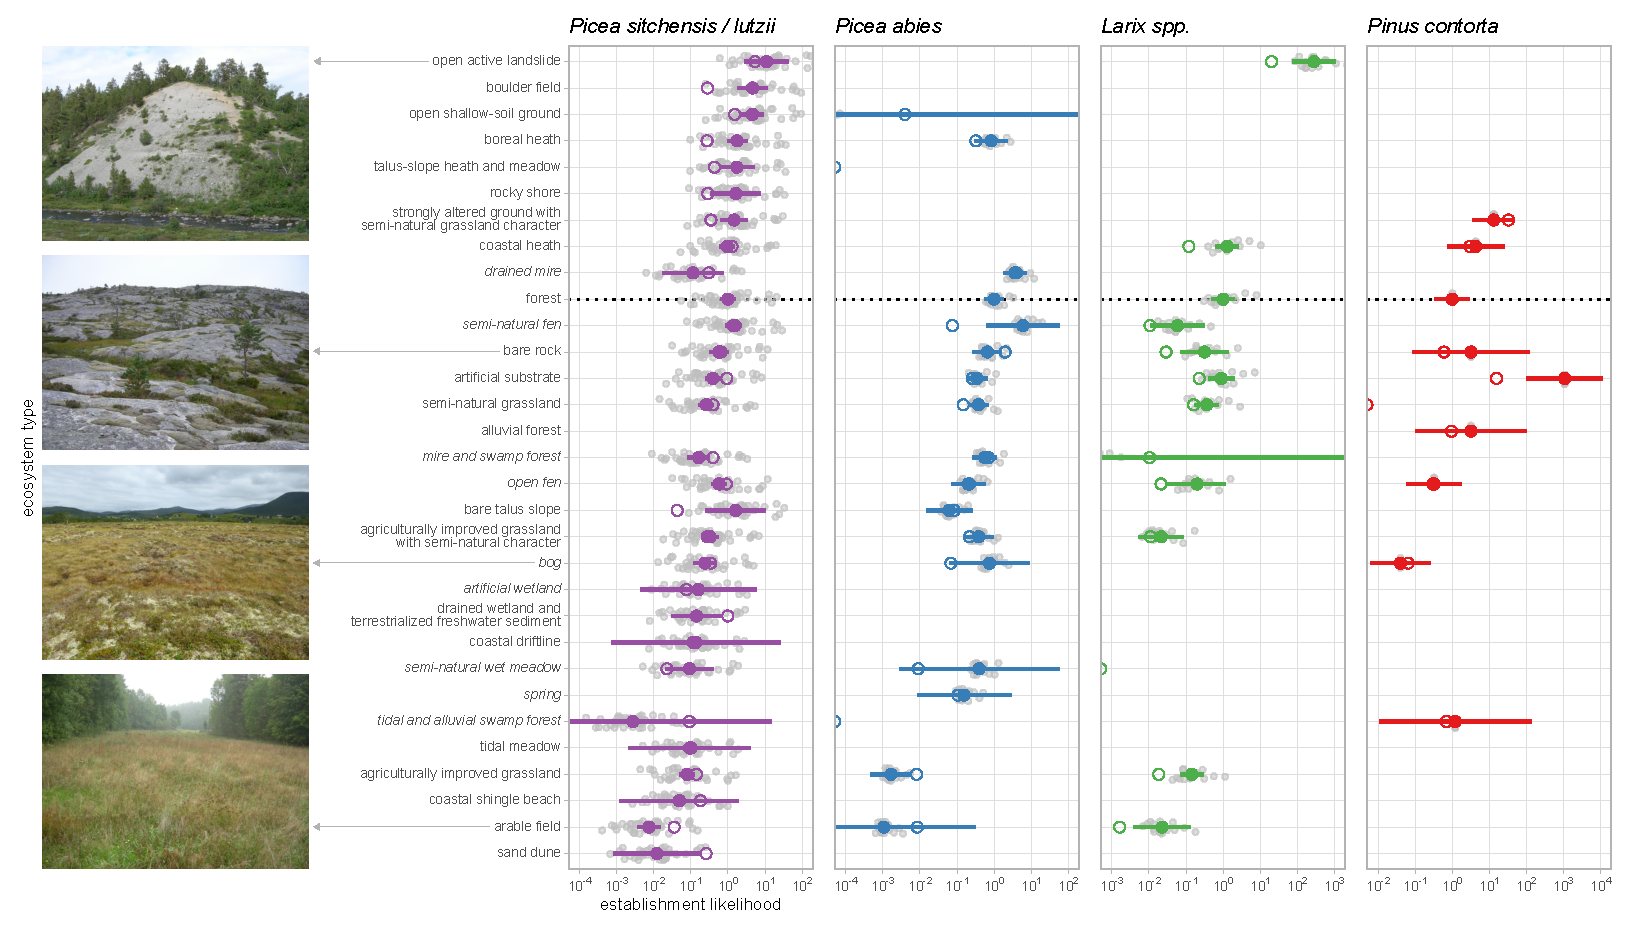
\includegraphics{/home/julien/Documents/dissertation/chapter3/conifer-plantation-spread/ms/figures/establishment/establishment.pdf}
\caption{\label{fig:establishment}Relative densities (unfilled points) and relative establishment likelihoods (filled points) of four alien conifer species groups in various ecosystem types, using `forest' as the reference level. Zero density is plotted at the lower limit of the x-axis. Estimates of relative establishment likelihood are shown with 95 \% confidence intervals. Grey point clouds depict relative establishment likelihoods for individual sites in our data set. The order of ecosystem types along the y-axis is determined by a confidence-weighted mean of their percentile-ranked establishment likelihoods within species, such that types with consistently high establishment likelihood across species are at the top. Wetland ecosystem types are shown in italic font. Ecosystem types without wildlings and covering less than one hectare across all sites for that species are not displayed. Photos licensed CC BY 4.0 Rune Halvorsen.}
\end{figure}

\end{landscape}

\newpage

Among ecosystems with at least one wildling, estimated establishment likelihoods varied by 3--5 orders of magnitude for the different species.
Patterns of relative establishment likelihood were modestly similar between species, with positive rank correlations in four of six species pairs (tab. \ref{tab:species-correlation-table}).

\begin{table}

\caption{\label{tab:species-correlation-table}Rank correlations of relative establishment likelihoods in ecosystem types, between pairs of species groups.}
\centering
\begin{tabular}[t]{>{}llll}
\toprule
\em{ } & \em{Picea abies} & \em{Larix spp.} & \em{Pinus contorta}\\
\midrule
\em{Picea sitchensis / lutzii} & 0.37 & 0.5 & 0.12\\
\em{Picea abies} &  & 0.18 & -0.1\\
\em{Larix spp.} &  &  & -0.1\\
\bottomrule
\end{tabular}
\end{table}

Variation in establishment likelihoods shrank when ecosystems were aggregated (by category or structuring process; fig.~\ref{fig:establishment-hypotheses}).
No more than two orders of magnitude separated the different groups.
Sitka/Lutz spruce and Norway spruce established at higher rates in wetland ecosystems than terrestrial ecosystems, while the opposite was true for larches and lodgepole pine.
Sitka/Lutz spruce and Norway spruce did not generally colonize disturbance-structured ecosystems at higher rates than ecosystems without disturbance structuring.
For larches and lodgepole pine, structuring by natural disturbance and anthropogenic disturbance, respectively, were associated with the highest establishment likelihoods.
Yet despite larger sample sizes, the mean establishment likelihood in any particular group was rarely clearly distinguishable from that in other groups.

\newpage
\begin{landscape}

\begin{figure}
\centering
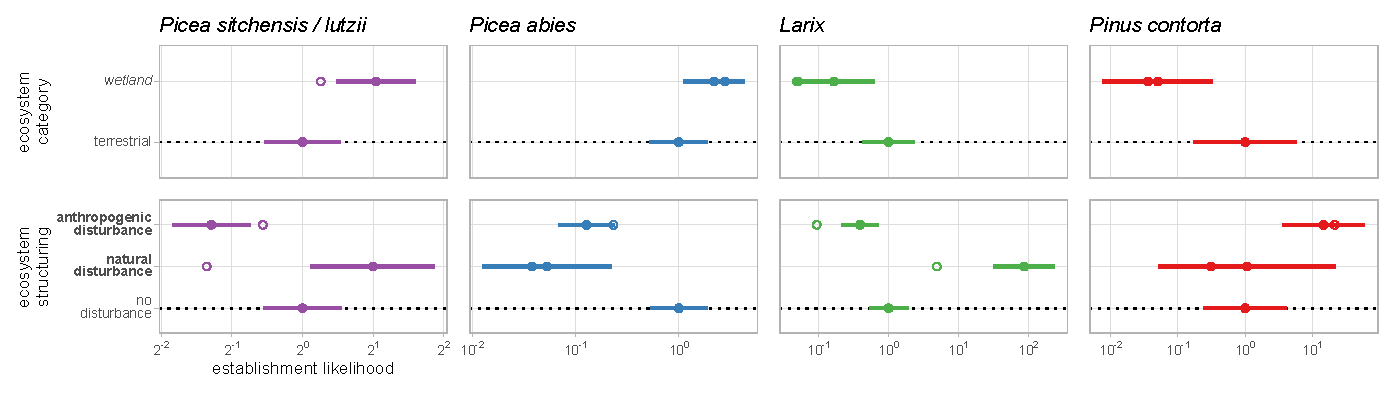
\includegraphics{/home/julien/Documents/dissertation/chapter3/conifer-plantation-spread/ms/figures/establishment-hypotheses.pdf}
\caption{\label{fig:establishment-hypotheses}Relative densities (unfilled points) and relative establishment likelihoods (filled points) of four alien conifer species groups among categories of ecosystem types (top) or structuring processes in ecosystem types (bottom). Estimates of relative establishment likelihood are shown with 95 \% confidence intervals. The horizontal dotted lines mark the reference level for the scaling. Strata without wildlings and covering less than one hectare across all sites for that species are not displayed.}
\end{figure}

\end{landscape}

\newpage

\hypertarget{discussion}{%
\section{Discussion}\label{discussion}}

\hypertarget{ecosystem-susceptibility}{%
\subsection{Ecosystem susceptibility}\label{ecosystem-susceptibility}}

In a large database of vegetation plots across Europe, Chytrý et al.(\protect\hyperlink{ref-chytryHabitatInvasionsAlien2008}{2008}\protect\hyperlink{ref-chytryHabitatInvasionsAlien2008}{b}) found that alien plants as a group are consistently found at low rates in mires and heaths, and high rates in arable, man-made, and coastal ecosystems.
The conifer species we examined --- perhaps with the exception of lodgepole pine --- do not conform to these broader trends in ecosystem invasibility.
Lodgepole pine establishment is relatively well studied, and our results are consistent with this literature.
``Bare rock'' harbors very few competitors and showed highest lodgepole pine establishment of all ecosystems (Despain \protect\hyperlink{ref-despainDispersalEcologyLodgepole2001}{2001}), ``coastal heath'' (a short shrubland) facilitated more establishment than grassland-like ecosystems (Taylor et al. \protect\hyperlink{ref-taylorDriversPlantInvasion2016}{2016}), all ecosystems with canopy cover were among those with lowest establishment (Taylor et al. \protect\hyperlink{ref-taylorDriversPlantInvasion2016}{2016}, Langdon et al. \protect\hyperlink{ref-langdonPinusContortaInvasion2010}{2010}), and ecosystems with high establishment were frequently structured by anthropogenic disturbance (Richardson et al. \protect\hyperlink{ref-richardsonPineInvasionsSouthern1994}{1994}).

It is difficult to evaluate our ecosystem susceptibility results against the recruitment patterns that have been described for the three other species.
For instance, Sitka spruce grows poorly under moisture stress and tolerates flooding well (Peterson et al. \protect\hyperlink{ref-petersonEcologyManagementSitka1997}{1997}), which might account for why it was twice as likely to establish in wetland ecosystems as in terrestrial ecosystems.
Yet it also established in ``open shallow-soil ground'' with very high likelihood, despite this ecosystem's characteristically dry soil.
This illustrates the trouble with deriving predictions for management units such as ecosystems from generalized statements about species autecology; should we expect few wildlings in ``open shallow-soil ground'' because it is dry, or many because it provides ample light and reduced competition (Peterson et al. \protect\hyperlink{ref-petersonEcologyManagementSitka1997}{1997})?
Furthermore, ecosystems that would seem inhospitable based on their overall characteristics may actually contain many localized opportunities for establishment, because seedling mortality is strongly regulated by microsites (Macek et al. \protect\hyperlink{ref-macekLifeDeathPicea2017}{2017}).
From this perspective, our estimates of establishment likelihood measure the density of suitable microsites in a given ecosystem.

The breadth in establishment likelihood suggests that differences between ecosystems deserve careful consideration when managing wildling spread.
This knowledge can be applied in at least two ways.
First, as a preventative measure, we recommend siting new plantations where surrounded by high proportions of ecosystems with low establishment likelihood.
In particular, ``arable fields'' harbor very few wildlings of any species and are common near existing plantations, so picking sites hemmed in by this kind of agricultural land should be both effective and feasible.
This would probably reduce the rate of wildling establishment by orders of magnitude, even if long distance dispersal might preclude complete containment (Albert et al. \protect\hyperlink{ref-albertLanduseChangeSubalpine2008}{2008}).
In some cases it may also be desirable to alter ecosystems adjacent to existing plantations to prevent (further) spread, for example by intensifying mowing regimes to promote the appearance of ``agriculturally improved grassland''.
Second, as a reactive measure, we recommend allocating resources for monitoring and control in proportion to relative ecosystem susceptibility.
Prioritizing ecosystems that are highly susceptible and also rare (e.g.~``open active landslide'') is especially likely to be cost-efficient.

The establishment patterns we quantify probably hold, more or less, beyond Norway (Chytrý et al. \protect\hyperlink{ref-chytryHabitatInvasionsAlien2008}{2008}\protect\hyperlink{ref-chytryHabitatInvasionsAlien2008}{b}).
From a manager's perspective, we expect that the ecosystems we report may translate well to equivalent types in similar classification systems, because the Nature in Norway classification is rule-based and aims for observer neutrality.
At the same time, we urge caution in extending our establishment estimates to ecosystems that are only broadly similar, because we found that similar types frequently showed markedly different susceptibility (e.g.~Norway spruce in ``agriculturally improved grassland with semi-natural character'' vs.~``agriculturally improved grassland'').

An observational study like ours informs management of long-lived, naturalized species more directly than experimental studies, because longer time frames are examined.
It measures long-term survival --- often the quantity of interest --- under a wide range of natural conditions experienced by the wildlings.
In contrast, seeding experiments generally observe only the youngest life stages, and the factors controlling individual success differ at later life stages (Dovčiak et al. \protect\hyperlink{ref-dovciakSeedRainEnvironmental2008}{2008}).
For example, Sitka spruce appears more likely to germinate in disturbed soil (Vikane et al. \protect\hyperlink{ref-vikaneInvasionCallunaHeath2013}{2013}), but less likely to survive there (Peterson et al. \protect\hyperlink{ref-petersonEcologyManagementSitka1997}{1997}).
On the other hand, experiments might be more useful when observed wildling spread is not representative of patterns in the wider landscape (e.g.~for species expanding from a single point of introduction).

\hypertarget{estimating-susceptibility}{%
\subsection{Estimating susceptibility}\label{estimating-susceptibility}}

Confounders of the relationship between ecosystem and wildling abundance caused wildling density to underestimate and sometimes completely mischaracterize differences in establishment likelihood between ecosystems.
The underestimation implies that confounding variables counteracted differences in ecosystem establishment in our sample --- for instance that susceptible ecosystems were concentrated at sites predicted to show limited establishment.
We caution, therefore, that direct inference from observations of wildling abundance misguides intuition about relative ecosystem susceptibility.
For example, the density of Sitka spruce wildlings was about equal in ``boreal heath'' and ``sand dunes'', but we estimate that establishment likelihood is actually about 100 times larger in ``boreal heath''.

Limitation: offset assumes that the spatial distribution of seed rain was no different when the plantation was younger and the trees shorter.
The effect size of WALD-modeled relative seed rain was estimated close to one for all species except Norway spruce, which indicates that spatial patterns of wildling abundance around plantations were captured satisfactorily by this variable.
We take this as evidence that the WALD model describes seed dispersal well in our system, but recognize that survivorship bias prevents rigorous assessment of this relationship with our data.
For example, the empirical seed dispersal model we tested generally showed a steeper decline in seed rain away from seed sources than the WALD model, so negative density dependence in seedling survival could skew the spatial distribution of wildling abundance towards the WALD model.
That this important covariate was modeled and not measured is a limitation of our method, and it makes the establishment likelihoods we estimate less certain.
Nevertheless, the mechanistic nature of the WALD model makes us more confident in its estimates across species and sites than we would be in a purely phenomenological model (Bullock et al. \protect\hyperlink{ref-bullockAllDispersalFunctions2018}{2018}).
Relative elevation's inconsistent effects on wildling abundance suggests that either terrain does not strongly affect seed dispersal or --- more likely --- vertical distance alone does a poor job of representing its effect.
In any case, there is no rule of thumb for management that wildlings tend to move up or down slopes.

We reiterate that our models do not estimate the total causal effect of climate on wildling abundance, because they set aside climate's influence on ecosystems (Westreich and Greenland \protect\hyperlink{ref-westreichTableFallacyPresenting2013}{2013}).
Therefore, we interpret the estimated climate effects with respect to physiological constraints within a given ecosystem.
The lack of a direct climate effect on Sitka/Lutz spruce wildling abundance is consistent with Sitka spruce's wide climatic tolerance relative to climatic variation in Norway (Peterson et al. \protect\hyperlink{ref-petersonEcologyManagementSitka1997}{1997}, Vollering et al. \protect\hyperlink{ref-volleringBunchingBackgroundBetters2019}{2019}, Appendix F).
Norway spruce seedling recruitment has previously been found to increase towards the wetter end of Norwegian climate (Tingstad et al. \protect\hyperlink{ref-tingstadTemperaturePrecipitationBiotic2015}{2015}), but most of our Norway spruce sites circumscribed a narrow part of that range.
We are not confident that lodgepole pine responds strongly to precipitation, as estimated, because the sample contained only six sites from two climates.

A curious feature of our results that needs more research is the large amount of unexplained variation in Sitka/Lutz spruce and lodgepole pine establishment likelihood between sites.
Our ability to predict these species' magnitude of spread at a specific site, relative to other sites, is still limited.
Ecosystem comparisons can nevertheless guide management.
Bianchi et al.~(\protect\hyperlink{ref-bianchiMethodsPredictingSitka2019}{2019}) struggled to predict regeneration density within Sitka spruce plantations from bare ground cover, moss cover, plantation age, and plantation density.
The inadequacy of plantation density as a predictor in this context suggests that the unexplained site-level variation in our models was not caused by differences in the densities of seed sources (which we assumed to be constant).
Alternative explanations could include: (1) property owners removing wildlings at some sites, or (2) differing demographic characteristics among plantations (Taylor et al. \protect\hyperlink{ref-taylorDriversPlantInvasion2016}{2016}), potentially as a result of provenance.

\hypertarget{generalizing-susceptibility}{%
\subsection{Generalizing susceptibility}\label{generalizing-susceptibility}}

The overarching characteristics that we used to aggregate ecosystems did a poor job of generalizing differences in susceptibility.
That is, groups of ecosystems belonging to the same hydrological category, or structured by the same form of disturbance, showed heterogeneous establishment likelihoods.
We note that slightly different sets of ecosystems comprised the groups for each species, depending on their presence in the data.
These differences in ecosystem composition help explain why the patterns of aggregated establishment likelihood varied between species.
This constraint hinders species comparisons but underlines our main takeaway from these results --- that the susceptibility of an individual ecosystem frequently diverges from those it is classified with.
Thus, we did not find any broad commonalities between susceptible ecosystems that could help guide wildling management where data are scarce.

Within species, we urge careful interpretation of the comparisons among ecosystem categories and structuring processes.
Many areas where conifer establishment is nearly impossible, like paved surfaces and annually plowed fields, count as terrestrial and anthropogenically disturbed, which lowers the relative establishment likelihood of these two groups.
Our results do not imply, for example, that any particular anthropogenic disturbance event will decrease establishment likelihood of Sitka/Lutz spruce relative to an ecosystem's prior state (indeed, Vikane et al.~(\protect\hyperlink{ref-vikaneInvasionCallunaHeath2013}{2013}) show that burning in coastal heathland increases Sitka spruce establishment).
Rather, we find that ecosystems structured by anthropogenic disturbance, on the whole, are no more susceptible to Sitka/Lutz spruce wildlings than other ecosystems.

\hypertarget{conclusions}{%
\section{Conclusions}\label{conclusions}}

Wildling spread from plantations is a growing problem (Richardson and Rejmánek \protect\hyperlink{ref-richardsonConifersInvasiveAliens2004}{2004}) and will probably worsen with recent pushes to increase tree planting worldwide (Brundu et al. \protect\hyperlink{ref-brunduGlobalGuidelinesSustainable2020}{2020}).
Meanwhile, remotely sensed and survey data are making detailed and accurate maps of ecosystems increasingly available over large extents (Horvath et al. \protect\hyperlink{ref-horvathDistributionModellingVegetation2019}{2019}), which presents opportunities to manage wildling spread more efficiently (Buckley et al. \protect\hyperlink{ref-buckleySlowingPineInvasion2005}{2005}).
Specifically, differences in ecosystem susceptibility can be leveraged to
reduce the rate of wildling establishment (potentially by orders of magnitude) through deliberate site selection for new plantations or targeted interventions around existing plantations.
However, managers should be cautious judging ecosystem susceptibility based on descriptions of the species' autecology, wildling densities, or generalizations about susceptibility across ecosystems.

One of main novelties of this study is that we inferred susceptibility/invasibility using mechanistically reconstructed, spatial estimates of seed rain.
Scientists studying invasibility at national and continental scales have already recognized the importance of normalizing observed levels of invasion by a spatially explicit estimate of exposure (i.e.~propagule pressure; Chytrý et al. \protect\hyperlink{ref-chytrySeparatingHabitatInvasibility2008}{2008}\protect\hyperlink{ref-chytrySeparatingHabitatInvasibility2008}{a}).
However, many studies quantifying ecosystem invasibility have not been able adjust for propagule pressure, typically because it is impossible to reconstruct the underlying dispersal history (Catford et al. \protect\hyperlink{ref-catfordQuantifyingLevelsBiological2012}{2012}).
We found that accounting for seed rain and other confounders of the relationship between ecosystems and wildling abundance underlined variation in ecosystem invasibility.

\hypertarget{authors-contributions}{%
\section{Authors' contributions}\label{authors-contributions}}

JV, SLO, and OSk conceived the ideas and designed methodology; SLO, LA, MOK, AO, JS, OSt, and ØS collected the data; JV analysed the data and led the writing of the manuscript. All authors contributed critically to the drafts and gave final approval for publication.

\hypertarget{acknowledgements}{%
\section{Acknowledgements}\label{acknowledgements}}

We thank Honorata Gajda, Knut Børge Strøm, Heidi Elin Myklebost, Jon Hagelin, Vigdis Frivoll, Sina Thu Randulff, Roy Mangersnes, Bjarne Homnes Oddane, Rune Søyland, Solbjørg Engen Torvik, Toralf Tysse, Craig Jackson, Miene-Marie Gastinger, Ola Westby Aamodt, and Anders Ringstad for their help in collecting and/or collating the field data.

\hypertarget{appendix}{%
\section{Appendix}\label{appendix}}

The WALD model takes the form of an inverse Gaussian distribution whose mean (\(\mu\)) and shape (\(\lambda\)) parameters are calculated from physical characteristics of the dispersal system:

\begin{equation}
\mu  = \frac{HU}{F}
\end{equation}
\begin{equation}
\lambda = \left(\frac{H}{\sigma}\right)^2
\end{equation}

where \(H\) is the seed release height, \(U\) is the mean horizontal wind velocity between \(H\) and the ground, \(F\) is the terminal velocity of the seed, and \(\sigma\) is a wind turbulence parameter.
We set \(H\) to the height of the central plantation, estimated \(U\) from a computed vertical wind profile, obtained \(F\) from literature, and calculated \(\sigma\) from an equation for turbulent flow as a function of vegetation height (eq. A4 in Skarpaas and Shea \protect\hyperlink{ref-skarpaasDispersalPatternsDispersal2007}{2007}).
We parameterized separate WALD models for 20º sectors around each seed source, to make seed dispersal anisotropic (directional).
In each sector we estimated mean vegetation height based on the composition of mapped ecosystem types (Appendix, table \ref{tab:types-table}).
Simultaneously, we randomly sampled 100 wind velocities in the direction of the sector during the species' dispersal season.
The 100 resulting WALD kernels produced the seed probability density in the sector, and individual sectors were weighed by the frequency of corresponding wind directions (again, during the species' dispersal season).
The wind data were obtained either from the nearest weather station (MET Norway), a 2.5 km resolution interpolated hindcast covering southern Norway (Haakenstad and Haugen \protect\hyperlink{ref-haakenstad15yearHighResolution2017}{2017}), or a 10 km resolution hindcast covering all of Norway (Reistad et al. \protect\hyperlink{ref-reistadHighresolutionHindcastWind2011}{2011}, Haakenstad et al. \protect\hyperlink{ref-haakenstadNORA10EIRevisedRegional2020}{2020}). We used weather station data if the station was less than 2.5 or 10 km away (depending on hindcast coverage), or else the highest resolution hindcast.

\begin{ThreePartTable}
\begin{TableNotes}
\item \textit{References: } 
\item 1. Harris, A. S. Sitka spruce. in Silvics of North America: 1. Conifers (eds. Burns, R. M. \& Honkala, B. H.) vol. 2 513–529 (U.S. Department of Agriculture, Forest Service, 1990).
\item 2. Sandvik, H. Kunnskapsstatus for spredning og effekter av fremmede bartrær på biologisk mangfold. (2012).
\item 3. Sullivan, J. Larix decidua. Fire Effects Information System, U.S. Department of Agriculture, Forest Service, Rocky Mountain Research Station,  Fire Sciences Laboratory https://www.fs.fed.us/database/feis/plants/tree/lardec/all.html (1994).
\item 4. Sullivan, J. Picea abies. Fire Effects Information System, U.S. Department of Agriculture, Forest Service, Rocky Mountain Research Station,  Fire Sciences Laboratory https://www.fs.fed.us/database/feis/plants/tree/picabi/all.html (1994).
\end{TableNotes}
\begin{longtable}[t]{>{}llll}
\caption{\label{tab:traits-table}Dispersal traits}\\
\toprule
species group & seed terminal velocity & dispersal season & references\\
\midrule
\em{Larix spp.} & 1.0 m/s & Dec - May & 2, 3\\
\em{Picea abies} & 0.58 m/s & Nov - May & 2, 4\\
\em{Pinus contorta} & 0.82 m/s & Sep - Dec & 2\\
\em{Picea sitchensis / lutzii} & 0.94 m/s & Oct - Feb & 1, 2\\
\bottomrule
\insertTableNotes
\end{longtable}
\end{ThreePartTable}

Some of the seed source polygons we registered in the field had distinctive features that we accounted for as follows.
Seed source polygons for which the species of interest only made up a fraction of the plantation composition (e.g.~in Olsen et al. \protect\hyperlink{ref-olsenKartleggingAvKortdistansespredning2019}{2019}) were used with their point source density adjusted accordingly.
For example, a plantation identified as composed of Sitka spruce and Norway spruce was assigned a seed source point density half that of a pure Sitka spruce plantation.
Likewise, `mixed forest' plantations (e.g.~in Appelgren \protect\hyperlink{ref-appelgrenKartleggingAvKortdistansespredning2018}{2018}) were assigned 0.1 times the seed source point density of a pure plantation.\\
Seed source polygons identified as logged (e.g.~in Appelgren \protect\hyperlink{ref-appelgrenKartleggingAvKortdistansespredning2018}{2018}) were included as seed sources only if we could confirm that they were logged no earlier the decade prior to mapping, using time series of aerial photos.

\begin{landscape}
\begin{longtable}[t]{l>{}llllllll}
\caption{\label{tab:sites-table}\label{tab:sites-table}Plantations}\\
\toprule
reference & species group & site & easting & northing & height & age & bio01\textsuperscript{a} & bio19\textsuperscript{b}\\
\midrule
\endfirsthead
\caption[]{\label{tab:sites-table}Plantations \textit{(continued)}}\\
\toprule
reference & species group & site & easting & northing & height & age & bio01\textsuperscript{a} & bio19\textsuperscript{b}\\
\midrule
\endhead

\endfoot
\bottomrule
\multicolumn{9}{l}{\rule{0pt}{1em}\textit{Note: }}\\
\multicolumn{9}{l}{\rule{0pt}{1em}Easting and Northing are given for UTM zone 33N. Height is given in meters and age in years.}\\
\multicolumn{9}{l}{\rule{0pt}{1em}\textsuperscript{a} mean annual temperature (°C)}\\
\multicolumn{9}{l}{\rule{0pt}{1em}\textsuperscript{b} precipitation in coldest quarter (cm)}\\
\multicolumn{9}{l}{\rule{0pt}{1em}\textsuperscript{*} interpolated as the mean height of other plantations of the same species, inversely weighted by difference in age}\\
\multicolumn{9}{l}{\rule{0pt}{1em}\textsuperscript{\dag} interpolated as the mean age of other plantations of the same species in the same region}\\
\endlastfoot
\cellcolor{gray!6}{Olsen et al. 2016} & \em{\cellcolor{gray!6}{Pinus contorta}} & \cellcolor{gray!6}{Fiskvikrokkdalen} & \cellcolor{gray!6}{292498} & \cellcolor{gray!6}{6843676} & \cellcolor{gray!6}{11} & \cellcolor{gray!6}{58} & \cellcolor{gray!6}{2.36} & \cellcolor{gray!6}{12.8}\\
Olsen et al. 2016 & \em{Pinus contorta} & Gulemyrane & 94625 & 7000110 & 9\textsuperscript{*} & 42 & 7.22 & 48.0\\
\cellcolor{gray!6}{Olsen et al. 2016} & \em{\cellcolor{gray!6}{Pinus contorta}} & \cellcolor{gray!6}{Selvik} & \cellcolor{gray!6}{74593} & \cellcolor{gray!6}{6978018} & \cellcolor{gray!6}{8} & \cellcolor{gray!6}{45} & \cellcolor{gray!6}{7.25} & \cellcolor{gray!6}{40.0}\\
Olsen et al. 2016 & \em{Pinus contorta} & Skarsheia & 78833 & 6979095 & 6 & 45 & 6.60 & 36.7\\
\cellcolor{gray!6}{Olsen et al. 2016} & \em{\cellcolor{gray!6}{Pinus contorta}} & \cellcolor{gray!6}{Sollitangen} & \cellcolor{gray!6}{260896} & \cellcolor{gray!6}{6859024} & \cellcolor{gray!6}{12} & \cellcolor{gray!6}{37} & \cellcolor{gray!6}{2.60} & \cellcolor{gray!6}{6.7}\\
\addlinespace
Olsen et al. 2016 & \em{Pinus contorta} & Tomasmyra & 260694 & 6864426 & 12 & 29 & 2.44 & 6.2\\
\cellcolor{gray!6}{Olsen et al. 2016} & \em{\cellcolor{gray!6}{Picea sitchensis / lutzii}} & \cellcolor{gray!6}{Gryttingdalen-vest} & \cellcolor{gray!6}{503887} & \cellcolor{gray!6}{7613803} & \cellcolor{gray!6}{8} & \cellcolor{gray!6}{52} & \cellcolor{gray!6}{4.56} & \cellcolor{gray!6}{49.0}\\
Olsen et al. 2016 & \em{Picea sitchensis / lutzii} & Gryttingdalen-oest & 504335 & 7613736 & 8 & 52 & 4.50 & 50.5\\
\cellcolor{gray!6}{Olsen et al. 2016} & \em{\cellcolor{gray!6}{Picea sitchensis / lutzii}} & \cellcolor{gray!6}{Holmsnes-nordvest} & \cellcolor{gray!6}{493935} & \cellcolor{gray!6}{7609464} & \cellcolor{gray!6}{11} & \cellcolor{gray!6}{49} & \cellcolor{gray!6}{5.36} & \cellcolor{gray!6}{45.3}\\
Olsen et al. 2016 & \em{Picea sitchensis / lutzii} & Holmsnes-soeroest & 494675 & 7608420 & 11 & 45 & 5.46 & 44.0\\
\addlinespace
\cellcolor{gray!6}{Olsen et al. 2016} & \em{\cellcolor{gray!6}{Picea sitchensis / lutzii}} & \cellcolor{gray!6}{Hov} & \cellcolor{gray!6}{496920} & \cellcolor{gray!6}{7608739} & \cellcolor{gray!6}{11} & \cellcolor{gray!6}{56} & \cellcolor{gray!6}{5.22} & \cellcolor{gray!6}{50.9}\\
Olsen et al. 2016 & \em{Picea sitchensis / lutzii} & Raavollmarka & 499105 & 7608885 & 18 & 59 & 4.80 & 51.1\\
\cellcolor{gray!6}{Appelgren and Torvik 2017} & \em{\cellcolor{gray!6}{Larix spp.}} & \cellcolor{gray!6}{Anisdal} & \cellcolor{gray!6}{-36439} & \cellcolor{gray!6}{6529890} & \cellcolor{gray!6}{22} & \cellcolor{gray!6}{56} & \cellcolor{gray!6}{7.37} & \cellcolor{gray!6}{38.8}\\
Appelgren and Torvik 2017 & \em{Larix spp.} & Haalandsbotn & -37108 & 6532830 & 20 & 57.5 & 7.00 & 38.9\\
\cellcolor{gray!6}{Appelgren and Torvik 2017} & \em{\cellcolor{gray!6}{Larix spp.}} & \cellcolor{gray!6}{Roeynaasen} & \cellcolor{gray!6}{-31279} & \cellcolor{gray!6}{6547997} & \cellcolor{gray!6}{25} & \cellcolor{gray!6}{77.5} & \cellcolor{gray!6}{6.88} & \cellcolor{gray!6}{36.5}\\
\addlinespace
Appelgren and Torvik 2017 & \em{Larix spp.} & Storemo & -107 & 6588189 & 23 & 60 & 7.15 & 33.0\\
\cellcolor{gray!6}{Appelgren and Torvik 2017} & \em{\cellcolor{gray!6}{Larix spp.}} & \cellcolor{gray!6}{Toegjefjellet} & \cellcolor{gray!6}{-22293} & \cellcolor{gray!6}{6546411} & \cellcolor{gray!6}{20} & \cellcolor{gray!6}{60} & \cellcolor{gray!6}{6.69} & \cellcolor{gray!6}{39.6}\\
Appelgren and Torvik 2017 & \em{Larix spp.} & Voren & -26899 & 6554824 & 20 & 62 & 6.42 & 39.6\\
\cellcolor{gray!6}{Appelgren and Torvik 2017} & \em{\cellcolor{gray!6}{Picea abies}} & \cellcolor{gray!6}{Mysingveien} & \cellcolor{gray!6}{-10547} & \cellcolor{gray!6}{6522150} & \cellcolor{gray!6}{21} & \cellcolor{gray!6}{52} & \cellcolor{gray!6}{6.34} & \cellcolor{gray!6}{53.9}\\
Appelgren and Torvik 2017 & \em{Picea abies} & Ollestad & -2440 & 6519912 & 20\textsuperscript{*} & 58 & 6.76 & 42.5\\
\addlinespace
\cellcolor{gray!6}{Appelgren and Torvik 2017} & \em{\cellcolor{gray!6}{Picea abies}} & \cellcolor{gray!6}{Varland} & \cellcolor{gray!6}{-15600} & \cellcolor{gray!6}{6584801} & \cellcolor{gray!6}{22} & \cellcolor{gray!6}{60} & \cellcolor{gray!6}{6.94} & \cellcolor{gray!6}{36.2}\\
Appelgren and Torvik 2017 & \em{Picea sitchensis / lutzii} & Dale & -30398 & 6586913 & 25 & 77 & 7.10 & 40.6\\
\cellcolor{gray!6}{Appelgren and Torvik 2017} & \em{\cellcolor{gray!6}{Picea sitchensis / lutzii}} & \cellcolor{gray!6}{Fjoesne} & \cellcolor{gray!6}{-11052} & \cellcolor{gray!6}{6650525} & \cellcolor{gray!6}{22} & \cellcolor{gray!6}{50} & \cellcolor{gray!6}{6.11} & \cellcolor{gray!6}{60.1}\\
Appelgren and Torvik 2017 & \em{Picea sitchensis / lutzii} & Kvia & -42603 & 6539369 & 20 & 57.5 & 8.02 & 30.6\\
\cellcolor{gray!6}{Appelgren and Torvik 2017} & \em{\cellcolor{gray!6}{Picea sitchensis / lutzii}} & \cellcolor{gray!6}{Roeynaasen} & \cellcolor{gray!6}{-31321} & \cellcolor{gray!6}{6548005} & \cellcolor{gray!6}{23} & \cellcolor{gray!6}{77.5} & \cellcolor{gray!6}{6.88} & \cellcolor{gray!6}{36.5}\\
\addlinespace
Appelgren and Torvik 2017 & \em{Picea sitchensis / lutzii} & Toegjefjellet & -22347 & 6546467 & 20 & 60 & 6.69 & 39.6\\
\cellcolor{gray!6}{Appelgren and Torvik 2017} & \em{\cellcolor{gray!6}{Picea sitchensis / lutzii}} & \cellcolor{gray!6}{Voren} & \cellcolor{gray!6}{-26991} & \cellcolor{gray!6}{6554850} & \cellcolor{gray!6}{18} & \cellcolor{gray!6}{52.5} & \cellcolor{gray!6}{6.42} & \cellcolor{gray!6}{39.6}\\
Appelgren and Torvik 2017 & \em{Picea sitchensis / lutzii} & Aarheia & -33443 & 6589861 & 28 & 60 & 7.31 & 38.2\\
\cellcolor{gray!6}{Kyrkjeeide et al. 2017} & \em{\cellcolor{gray!6}{Picea abies}} & \cellcolor{gray!6}{Myklebostad} & \cellcolor{gray!6}{481205} & \cellcolor{gray!6}{7469940} & \cellcolor{gray!6}{20\textsuperscript{*}} & \cellcolor{gray!6}{97} & \cellcolor{gray!6}{4.99} & \cellcolor{gray!6}{24.9}\\
Kyrkjeeide et al. 2017 & \em{Picea abies} & Tennes & 668660 & 7695332 & 20\textsuperscript{*} & 87 & 1.87 & 18.6\\
\addlinespace
\cellcolor{gray!6}{Kyrkjeeide et al. 2017} & \em{\cellcolor{gray!6}{Picea sitchensis / lutzii}} & \cellcolor{gray!6}{Hagheia} & \cellcolor{gray!6}{445925} & \cellcolor{gray!6}{7560670} & \cellcolor{gray!6}{18\textsuperscript{*}} & \cellcolor{gray!6}{55} & \cellcolor{gray!6}{4.89} & \cellcolor{gray!6}{49.4}\\
Kyrkjeeide et al. 2017 & \em{Picea sitchensis / lutzii} & Harteigen & 449285 & 7559665 & 15\textsuperscript{*} & 51.5 & 5.38 & 48.4\\
\cellcolor{gray!6}{Kyrkjeeide et al. 2017} & \em{\cellcolor{gray!6}{Picea sitchensis / lutzii}} & \cellcolor{gray!6}{Haakoeya} & \cellcolor{gray!6}{647074} & \cellcolor{gray!6}{7731726} & \cellcolor{gray!6}{17\textsuperscript{*}} & \cellcolor{gray!6}{42\textsuperscript{\dag}} & \cellcolor{gray!6}{3.16} & \cellcolor{gray!6}{30.0}\\
Appelgren 2018 & \em{Larix spp.} & Engjane & -34540 & 6529860 & 15 & 45 & 7.19 & 40.3\\
\cellcolor{gray!6}{Appelgren 2018} & \em{\cellcolor{gray!6}{Larix spp.}} & \cellcolor{gray!6}{Hyljafjellet} & \cellcolor{gray!6}{-34030} & \cellcolor{gray!6}{6529963} & \cellcolor{gray!6}{15} & \cellcolor{gray!6}{45} & \cellcolor{gray!6}{7.30} & \cellcolor{gray!6}{39.6}\\
\addlinespace
Appelgren 2018 & \em{Larix spp.} & Hoegaas & -25415 & 6560056 & 20 & 57.5 & 6.77 & 38.8\\
\cellcolor{gray!6}{Appelgren 2018} & \em{\cellcolor{gray!6}{Larix spp.}} & \cellcolor{gray!6}{Myrvoll} & \cellcolor{gray!6}{-12944} & \cellcolor{gray!6}{6522033} & \cellcolor{gray!6}{12} & \cellcolor{gray!6}{17.5} & \cellcolor{gray!6}{7.06} & \cellcolor{gray!6}{43.4}\\
Appelgren 2018 & \em{Larix spp.} & Oaland & -7652 & 6563045 & 17 & 52.5 & 5.48 & 49.7\\
\cellcolor{gray!6}{Appelgren 2018} & \em{\cellcolor{gray!6}{Picea abies}} & \cellcolor{gray!6}{Efteland} & \cellcolor{gray!6}{-15304} & \cellcolor{gray!6}{6523548} & \cellcolor{gray!6}{20} & \cellcolor{gray!6}{45} & \cellcolor{gray!6}{6.69} & \cellcolor{gray!6}{53.8}\\
Appelgren 2018 & \em{Picea abies} & Myrvoll & -13000 & 6522143 & 18 & 71.5 & 7.06 & 43.4\\
\addlinespace
\cellcolor{gray!6}{Appelgren 2018} & \em{\cellcolor{gray!6}{Picea sitchensis / lutzii}} & \cellcolor{gray!6}{Foersvoll} & \cellcolor{gray!6}{-29434} & \cellcolor{gray!6}{6588711} & \cellcolor{gray!6}{24} & \cellcolor{gray!6}{54} & \cellcolor{gray!6}{7.22} & \cellcolor{gray!6}{37.7}\\
Appelgren 2018 & \em{Picea sitchensis / lutzii} & Hommeland & -17515 & 6559100 & 17 & 47 & 6.01 & 40.1\\
\cellcolor{gray!6}{Appelgren 2018} & \em{\cellcolor{gray!6}{Picea sitchensis / lutzii}} & \cellcolor{gray!6}{Hyljafjellet} & \cellcolor{gray!6}{-34044} & \cellcolor{gray!6}{6529954} & \cellcolor{gray!6}{13.5} & \cellcolor{gray!6}{45} & \cellcolor{gray!6}{7.30} & \cellcolor{gray!6}{39.6}\\
Appelgren 2018 & \em{Picea sitchensis / lutzii} & Oaland & -7648 & 6563033 & 15 & 52.5 & 5.48 & 49.7\\
\cellcolor{gray!6}{Appelgren 2018} & \em{\cellcolor{gray!6}{Picea sitchensis / lutzii}} & \cellcolor{gray!6}{Sandve} & \cellcolor{gray!6}{-58701} & \cellcolor{gray!6}{6601600} & \cellcolor{gray!6}{11} & \cellcolor{gray!6}{30} & \cellcolor{gray!6}{7.83} & \cellcolor{gray!6}{38.8}\\
\addlinespace
Appelgren 2018 & \em{Picea sitchensis / lutzii} & Skorphella & -30767 & 6581293 & 13 & 35 & 7.87 & 31.3\\
\cellcolor{gray!6}{Appelgren 2018} & \em{\cellcolor{gray!6}{Picea sitchensis / lutzii}} & \cellcolor{gray!6}{Starebakkane} & \cellcolor{gray!6}{-43287} & \cellcolor{gray!6}{6563381} & \cellcolor{gray!6}{18} & \cellcolor{gray!6}{52.5} & \cellcolor{gray!6}{8.08} & \cellcolor{gray!6}{27.9}\\
Appelgren 2018 & \em{Picea sitchensis / lutzii} & Veggjaberget & -35788 & 6526000 & 12 & 27.5 & 8.04 & 35.0\\
\cellcolor{gray!6}{Appelgren 2018} & \em{\cellcolor{gray!6}{Picea sitchensis / lutzii}} & \cellcolor{gray!6}{Vikra} & \cellcolor{gray!6}{-59126} & \cellcolor{gray!6}{6601266} & \cellcolor{gray!6}{22\textsuperscript{*}} & \cellcolor{gray!6}{78} & \cellcolor{gray!6}{7.97} & \cellcolor{gray!6}{37.5}\\
Olsen et al. 2019 & \em{Larix spp.} & Stordalslia & 418827 & 7303180 & 11.9 & 16.5 & 4.62 & 52.2\\
\addlinespace
\cellcolor{gray!6}{Olsen et al. 2019} & \em{\cellcolor{gray!6}{Picea abies}} & \cellcolor{gray!6}{Storbergan} & \cellcolor{gray!6}{413255} & \cellcolor{gray!6}{7349964} & \cellcolor{gray!6}{13.1} & \cellcolor{gray!6}{49} & \cellcolor{gray!6}{5.02} & \cellcolor{gray!6}{55.6}\\
Olsen et al. 2019 & \em{Picea abies} & Svinnes & 385625 & 7306386 & 15.3 & 36.5 & 5.57 & 41.0\\
\cellcolor{gray!6}{Olsen et al. 2019} & \em{\cellcolor{gray!6}{Picea sitchensis / lutzii}} & \cellcolor{gray!6}{Alstahaugmyran} & \cellcolor{gray!6}{382564} & \cellcolor{gray!6}{7311547} & \cellcolor{gray!6}{15.7} & \cellcolor{gray!6}{31.5} & \cellcolor{gray!6}{5.49} & \cellcolor{gray!6}{45.7}\\
Olsen et al. 2019 & \em{Picea sitchensis / lutzii} & Hamran & 373448 & 7266074 & 17.2 & 26 & 5.69 & 42.3\\
\cellcolor{gray!6}{Olsen et al. 2019} & \em{\cellcolor{gray!6}{Picea sitchensis / lutzii}} & \cellcolor{gray!6}{Langvassfjellet} & \cellcolor{gray!6}{409484} & \cellcolor{gray!6}{7330371} & \cellcolor{gray!6}{17.6} & \cellcolor{gray!6}{36.5} & \cellcolor{gray!6}{4.87} & \cellcolor{gray!6}{54.0}\\
\addlinespace
Olsen et al. 2019 & \em{Picea sitchensis / lutzii} & Meaasen & 386111 & 7333724 & 14.1 & 43.5 & 5.70 & 34.5\\
\cellcolor{gray!6}{Olsen et al. 2019} & \em{\cellcolor{gray!6}{Picea sitchensis / lutzii}} & \cellcolor{gray!6}{Myrmo} & \cellcolor{gray!6}{391075} & \cellcolor{gray!6}{7321058} & \cellcolor{gray!6}{18.8} & \cellcolor{gray!6}{37} & \cellcolor{gray!6}{5.22} & \cellcolor{gray!6}{37.4}\\
Olsen et al. 2019 & \em{Picea sitchensis / lutzii} & Olabergan & 410600 & 7341996 & 18.8 & 29 & 5.31 & 45.0\\
\cellcolor{gray!6}{Olsen et al. 2019} & \em{\cellcolor{gray!6}{Picea sitchensis / lutzii}} & \cellcolor{gray!6}{Plogskjaeret} & \cellcolor{gray!6}{378814} & \cellcolor{gray!6}{7280849} & \cellcolor{gray!6}{16.1} & \cellcolor{gray!6}{26} & \cellcolor{gray!6}{5.57} & \cellcolor{gray!6}{43.5}\\
Olsen et al. 2019 & \em{Picea sitchensis / lutzii} & Sandmoan & 382107 & 7329122 & 10.8 & 33 & 5.73 & 33.7\\
\addlinespace
\cellcolor{gray!6}{Olsen et al. 2019} & \em{\cellcolor{gray!6}{Picea sitchensis / lutzii}} & \cellcolor{gray!6}{Steinaasen} & \cellcolor{gray!6}{375834} & \cellcolor{gray!6}{7274496} & \cellcolor{gray!6}{17.9} & \cellcolor{gray!6}{35} & \cellcolor{gray!6}{5.50} & \cellcolor{gray!6}{37.6}\\
Olsen et al. 2019 & \em{Picea sitchensis / lutzii} & Svinnes & 385652 & 7306426 & 16.4 & 37.5 & 5.65 & 40.1\\
\cellcolor{gray!6}{Olsen et al. 2019} & \em{\cellcolor{gray!6}{Picea sitchensis / lutzii}} & \cellcolor{gray!6}{Valan} & \cellcolor{gray!6}{383545} & \cellcolor{gray!6}{7304119} & \cellcolor{gray!6}{15.5} & \cellcolor{gray!6}{35} & \cellcolor{gray!6}{5.61} & \cellcolor{gray!6}{41.5}\\
Sandven et al. 2019 & \em{Larix spp.} & Ytre-bjotveit & 49799 & 6729344 & 19.4 & 72 & 5.52 & 34.5\\
\cellcolor{gray!6}{Sandven et al. 2019} & \em{\cellcolor{gray!6}{Larix spp.}} & \cellcolor{gray!6}{Knappeidet} & \cellcolor{gray!6}{-47542} & \cellcolor{gray!6}{6737678} & \cellcolor{gray!6}{17.2} & \cellcolor{gray!6}{32} & \cellcolor{gray!6}{7.99} & \cellcolor{gray!6}{39.4}\\
\addlinespace
Sandven et al. 2019 & \em{Larix spp.} & Indre-bjotveit & 51174 & 6730928 & 24.5 & 84 & 5.82 & 35.9\\
\cellcolor{gray!6}{Sandven et al. 2019} & \em{\cellcolor{gray!6}{Picea abies}} & \cellcolor{gray!6}{Boerve} & \cellcolor{gray!6}{37746} & \cellcolor{gray!6}{6711673} & \cellcolor{gray!6}{31.9} & \cellcolor{gray!6}{64} & \cellcolor{gray!6}{5.49} & \cellcolor{gray!6}{46.6}\\
Sandven et al. 2019 & \em{Picea abies} & Skare & 31612 & 6676392 & 22 & 66 & 4.41 & 50.6\\
\cellcolor{gray!6}{Sandven et al. 2019} & \em{\cellcolor{gray!6}{Picea abies}} & \cellcolor{gray!6}{Oeystese} & \cellcolor{gray!6}{16634} & \cellcolor{gray!6}{6726920} & \cellcolor{gray!6}{15.6} & \cellcolor{gray!6}{57} & \cellcolor{gray!6}{6.42} & \cellcolor{gray!6}{67.4}\\
Sandven et al. 2019 & \em{Picea abies} & Vasshjallane & 65573 & 6728437 & 22.8 & 56 & 5.53 & 29.8\\
\addlinespace
\cellcolor{gray!6}{Sandven et al. 2019} & \em{\cellcolor{gray!6}{Picea abies}} & \cellcolor{gray!6}{Hjelmtveit} & \cellcolor{gray!6}{-31407} & \cellcolor{gray!6}{6756542} & \cellcolor{gray!6}{21.4} & \cellcolor{gray!6}{57} & \cellcolor{gray!6}{7.15} & \cellcolor{gray!6}{57.3}\\
Sandven et al. 2019 & \em{Picea abies} & Bondhusdalen & 15726 & 6695404 & 16.2 & 55 & 5.67 & 44.0\\
\cellcolor{gray!6}{Sandven et al. 2019} & \em{\cellcolor{gray!6}{Picea abies}} & \cellcolor{gray!6}{Saeboe} & \cellcolor{gray!6}{-36690} & \cellcolor{gray!6}{6759365} & \cellcolor{gray!6}{21.2} & \cellcolor{gray!6}{51} & \cellcolor{gray!6}{7.07} & \cellcolor{gray!6}{59.8}\\
Sandven et al. 2019 & \em{Picea abies} & Indre-arna & -25457 & 6738087 & 14.4 & 52 & 6.94 & 45.2\\
\cellcolor{gray!6}{Sandven et al. 2019} & \em{\cellcolor{gray!6}{Picea abies}} & \cellcolor{gray!6}{Kvamskogen} & \cellcolor{gray!6}{4982} & \cellcolor{gray!6}{6726838} & \cellcolor{gray!6}{20.4} & \cellcolor{gray!6}{101} & \cellcolor{gray!6}{4.98} & \cellcolor{gray!6}{57.1}\\
\addlinespace
Sandven et al. 2019 & \em{Picea abies} & Rosendal & -1965 & 6685031 & 16.8 & 49 & 6.94 & 55.3\\
\cellcolor{gray!6}{Sandven et al. 2019} & \em{\cellcolor{gray!6}{Picea sitchensis / lutzii}} & \cellcolor{gray!6}{Midtre-fjell} & \cellcolor{gray!6}{-47585} & \cellcolor{gray!6}{6729572} & \cellcolor{gray!6}{23.5} & \cellcolor{gray!6}{50} & \cellcolor{gray!6}{7.74} & \cellcolor{gray!6}{44.8}\\
Sandven et al. 2019 & \em{Picea sitchensis / lutzii} & Oevre-manger & -43485 & 6764574 & 17.5 & 46 & 7.78 & 53.3\\
\cellcolor{gray!6}{Sandven et al. 2019} & \em{\cellcolor{gray!6}{Picea sitchensis / lutzii}} & \cellcolor{gray!6}{Fuglavasstoppen} & \cellcolor{gray!6}{-50243} & \cellcolor{gray!6}{6740596} & \cellcolor{gray!6}{19.5} & \cellcolor{gray!6}{48} & \cellcolor{gray!6}{7.86} & \cellcolor{gray!6}{46.0}\\
Sandven et al. 2019 & \em{Picea sitchensis / lutzii} & Kvitefjella & -48847 & 6730154 & 21.1 & 50 & 7.57 & 47.6\\
\addlinespace
\cellcolor{gray!6}{Sandven et al. 2019} & \em{\cellcolor{gray!6}{Picea sitchensis / lutzii}} & \cellcolor{gray!6}{Kausland} & \cellcolor{gray!6}{-50236} & \cellcolor{gray!6}{6718477} & \cellcolor{gray!6}{22.2} & \cellcolor{gray!6}{44} & \cellcolor{gray!6}{7.84} & \cellcolor{gray!6}{46.2}\\
Sandven et al. 2019 & \em{Picea sitchensis / lutzii} & Misje & -51009 & 6743828 & 20.8 & 54 & 7.99 & 45.1\\*
\end{longtable}
\end{landscape}

\begin{landscape}
\begin{longtable}[t]{llllr}
\caption{\label{tab:types-table}\label{tab:types-table}Ecosystem types}\\
\toprule
type & code & category & structuring & vegetation height\textsuperscript{a}\\
\midrule
\endfirsthead
\caption[]{\label{tab:types-table}Ecosystem types \textit{(continued)}}\\
\toprule
type & code & category & structuring & vegetation height\textsuperscript{a}\\
\midrule
\endhead

\endfoot
\bottomrule
\multicolumn{5}{l}{\rule{0pt}{1em}\textsuperscript{a} approximate vegetation heights (meters) are used only to estimate wind turbulence}\\
\endlastfoot
\cellcolor{gray!6}{bare rock} & \cellcolor{gray!6}{T1} & \cellcolor{gray!6}{terrestrial} & \cellcolor{gray!6}{} & \cellcolor{gray!6}{0.0}\\
open shallow-soil ground & T2 & terrestrial &  & 0.5\\
\cellcolor{gray!6}{arctic-alpine heath and lee side} & \cellcolor{gray!6}{T3} & \cellcolor{gray!6}{terrestrial} & \cellcolor{gray!6}{} & \cellcolor{gray!6}{0.5}\\
forest & T4 & terrestrial &  & 10.0\\
\cellcolor{gray!6}{rocky shore} & \cellcolor{gray!6}{T6} & \cellcolor{gray!6}{terrestrial} & \cellcolor{gray!6}{environmental stress} & \cellcolor{gray!6}{0.0}\\
\addlinespace
tidal meadow & T12 & terrestrial & environmental stress & 0.5\\
\cellcolor{gray!6}{bare talus slope} & \cellcolor{gray!6}{T13} & \cellcolor{gray!6}{terrestrial} & \cellcolor{gray!6}{regulating disturbance} & \cellcolor{gray!6}{0.0}\\
talus-slope heath and meadow & T16 & terrestrial & regulating disturbance & 0.5\\
\cellcolor{gray!6}{open active landslide} & \cellcolor{gray!6}{T17} & \cellcolor{gray!6}{terrestrial} & \cellcolor{gray!6}{destabilizing disturbance} & \cellcolor{gray!6}{0.0}\\
open alluvial sediment & T18 & terrestrial & destabilizing disturbance & 0.0\\
\addlinespace
\cellcolor{gray!6}{sand dune} & \cellcolor{gray!6}{T21} & \cellcolor{gray!6}{terrestrial} & \cellcolor{gray!6}{destabilizing disturbance} & \cellcolor{gray!6}{0.0}\\
coastal driftline & T24 & terrestrial & destabilizing disturbance & 0.5\\
\cellcolor{gray!6}{boulder field} & \cellcolor{gray!6}{T27} & \cellcolor{gray!6}{terrestrial} & \cellcolor{gray!6}{regulating disturbance} & \cellcolor{gray!6}{0.0}\\
coastal shingle beach & T29 & terrestrial & regulating disturbance & 0.0\\
\cellcolor{gray!6}{alluvial forest} & \cellcolor{gray!6}{T30} & \cellcolor{gray!6}{terrestrial} & \cellcolor{gray!6}{destabilizing disturbance} & \cellcolor{gray!6}{10.0}\\
\addlinespace
boreal heath & T31 & terrestrial & moderate anthropogenic disturbance & 0.5\\
\cellcolor{gray!6}{semi-natural grassland} & \cellcolor{gray!6}{T32} & \cellcolor{gray!6}{terrestrial} & \cellcolor{gray!6}{moderate anthropogenic disturbance} & \cellcolor{gray!6}{0.5}\\
semi-natural tidal and salt meadow & T33 & terrestrial & moderate anthropogenic disturbance & 0.5\\
\cellcolor{gray!6}{coastal heath} & \cellcolor{gray!6}{T34} & \cellcolor{gray!6}{terrestrial} & \cellcolor{gray!6}{moderate anthropogenic disturbance} & \cellcolor{gray!6}{0.5}\\
artificial substrate & T35 & terrestrial & strong anthropogenic disturbance & 0.0\\
\addlinespace
\cellcolor{gray!6}{artificial substrate} & \cellcolor{gray!6}{T37} & \cellcolor{gray!6}{terrestrial} & \cellcolor{gray!6}{strong anthropogenic disturbance} & \cellcolor{gray!6}{0.0}\\
artificial substrate & T39 & terrestrial & strong anthropogenic disturbance & 0.0\\
\cellcolor{gray!6}{artificial substrate} & \cellcolor{gray!6}{T43} & \cellcolor{gray!6}{terrestrial} & \cellcolor{gray!6}{strong anthropogenic disturbance} & \cellcolor{gray!6}{0.0}\\
drained wetland and terrestrialized freshwater sediment & T36 & terrestrial & strong anthropogenic disturbance & 0.5\\
\cellcolor{gray!6}{tree plantation} & \cellcolor{gray!6}{T38} & \cellcolor{gray!6}{terrestrial} & \cellcolor{gray!6}{strong anthropogenic disturbance} & \cellcolor{gray!6}{10.0}\\
\addlinespace
strongly altered ground with semi-natural grassland character & T40 & terrestrial & strong anthropogenic disturbance & 0.0\\
\cellcolor{gray!6}{agriculturally improved grassland with semi-natural character} & \cellcolor{gray!6}{T41} & \cellcolor{gray!6}{terrestrial} & \cellcolor{gray!6}{strong anthropogenic disturbance} & \cellcolor{gray!6}{0.5}\\
landscaped patch or field & T42 & terrestrial & strong anthropogenic disturbance & 0.0\\
\cellcolor{gray!6}{arable field} & \cellcolor{gray!6}{T44} & \cellcolor{gray!6}{terrestrial} & \cellcolor{gray!6}{strong anthropogenic disturbance} & \cellcolor{gray!6}{0.5}\\
agriculturally improved grassland & T45 & terrestrial & strong anthropogenic disturbance & 0.5\\
\addlinespace
\cellcolor{gray!6}{open fen} & \cellcolor{gray!6}{V1} & \cellcolor{gray!6}{wetland} & \cellcolor{gray!6}{} & \cellcolor{gray!6}{0.0}\\
mire and swamp forest & V2 & wetland &  & 10.0\\
\cellcolor{gray!6}{bog} & \cellcolor{gray!6}{V3} & \cellcolor{gray!6}{wetland} & \cellcolor{gray!6}{environmental stress} & \cellcolor{gray!6}{0.0}\\
spring & V4 & wetland & environmental stress & 0.0\\
\cellcolor{gray!6}{tidal and alluvial swamp forest} & \cellcolor{gray!6}{V8} & \cellcolor{gray!6}{wetland} & \cellcolor{gray!6}{environmental stress} & \cellcolor{gray!6}{10.0}\\
\addlinespace
semi-natural fen & V9 & wetland & moderate anthropogenic disturbance & 0.0\\
\cellcolor{gray!6}{semi-natural wet meadow} & \cellcolor{gray!6}{V10} & \cellcolor{gray!6}{wetland} & \cellcolor{gray!6}{moderate anthropogenic disturbance} & \cellcolor{gray!6}{0.0}\\
peat quarry & V11 & wetland & strong anthropogenic disturbance & 0.0\\
\cellcolor{gray!6}{drained mire} & \cellcolor{gray!6}{V12} & \cellcolor{gray!6}{wetland} & \cellcolor{gray!6}{strong anthropogenic disturbance} & \cellcolor{gray!6}{0.0}\\
artificial wetland & V13 & wetland & strong anthropogenic disturbance & 0.0\\*
\end{longtable}
\end{landscape}

\begin{table}

\caption{\label{tab:model-comparison-table}Comparison of models with different seed dispersal estimates}
\centering
\begin{tabular}[t]{llrrr}
\toprule
species group & seed dispersal estimate & AIC & dAIC & df\\
\midrule
 & WALD & 51967.261 & 0.0000 & 38\\

 & Exponential Power & 128861.239 & 76893.9779 & 38\\

\multirow{-3}{*}{\raggedright\arraybackslash Picea sitchensis / lutzii} & none & 54477.712 & 2510.4515 & 38\\
\cmidrule{1-5}
 & WALD & 9680.586 & 0.0000 & 26\\

 & Exponential Power & 25316.450 & 15635.8645 & 26\\

\multirow{-3}{*}{\raggedright\arraybackslash Picea abies} & none & 9781.127 & 100.5414 & 26\\
\cmidrule{1-5}
 & WALD & 10057.588 & 0.0000 & 21\\

\multirow{-2}{*}{\raggedright\arraybackslash Larix} & Exponential Power & 27310.048 & 17252.4596 & 21\\
\cmidrule{1-5}
 & WALD & 3319.143 & 0.0000 & 17\\

 & Exponential Power & NA & NA & 17\\

\multirow{-3}{*}{\raggedright\arraybackslash Pinus contorta} & none & 3372.102 & 52.9581 & 17\\
\bottomrule
\end{tabular}
\end{table}

\begin{longtable}[t]{lrrrr}
\caption{\label{tab:summaries-tables}\label{tab:Ps}Model summary for Picea sitchensis / lutzii. The conditional submodel is glmmTMB's genpois (Generalized Poisson) family with dispersion parameter phi² = 7.745472}\\
\toprule
\multicolumn{1}{c}{ } & \multicolumn{2}{c}{Fixed effects} & \multicolumn{2}{c}{Random effects} \\
\cmidrule(l{3pt}r{3pt}){2-3} \cmidrule(l{3pt}r{3pt}){4-5}
Term & Estimate & 95\% CI & SD (Intercept) & N\\
\midrule
\addlinespace[0.3em]
\multicolumn{5}{l}{\textbf{Conditional model}}\\
\hspace{1em}\cellcolor{gray!6}{Intercept} & \cellcolor{gray!6}{-1.80} & \cellcolor{gray!6}{-2.28, -1.31} & \cellcolor{gray!6}{} & \cellcolor{gray!6}{}\\
\hspace{1em}age & -0.08 & -0.54, 0.38 &  & \\
\hspace{1em}\cellcolor{gray!6}{bio01} & \cellcolor{gray!6}{0.54} & \cellcolor{gray!6}{0.01, 1.08} & \cellcolor{gray!6}{} & \cellcolor{gray!6}{}\\
\hspace{1em}bio19 & -0.03 & -0.55, 0.5 &  & \\
\hspace{1em}\cellcolor{gray!6}{relelev} & \cellcolor{gray!6}{-0.12} & \cellcolor{gray!6}{-0.19, -0.05} & \cellcolor{gray!6}{} & \cellcolor{gray!6}{}\\
\hspace{1em}T45 & -2.25 & -2.42, -2.08 &  & \\
\hspace{1em}\cellcolor{gray!6}{artificial} & \cellcolor{gray!6}{-1.07} & \cellcolor{gray!6}{-1.27, -0.87} & \cellcolor{gray!6}{} & \cellcolor{gray!6}{}\\
\hspace{1em}T44 & -4.90 & -5.68, -4.12 &  & \\
\hspace{1em}\cellcolor{gray!6}{T32} & \cellcolor{gray!6}{-1.24} & \cellcolor{gray!6}{-1.42, -1.06} & \cellcolor{gray!6}{} & \cellcolor{gray!6}{}\\
\hspace{1em}V9 & 0.84 & 0.63, 1.05 &  & \\
\hspace{1em}\cellcolor{gray!6}{T34} & \cellcolor{gray!6}{0.15} & \cellcolor{gray!6}{0.01, 0.29} & \cellcolor{gray!6}{} & \cellcolor{gray!6}{}\\
\hspace{1em}V12 & -0.37 & -1.92, 1.19 &  & \\
\hspace{1em}\cellcolor{gray!6}{V1} & \cellcolor{gray!6}{-0.37} & \cellcolor{gray!6}{-0.53, -0.22} & \cellcolor{gray!6}{} & \cellcolor{gray!6}{}\\
\hspace{1em}T13 & 2.13 & 0.57, 3.7 &  & \\
\hspace{1em}\cellcolor{gray!6}{T41} & \cellcolor{gray!6}{-1.12} & \cellcolor{gray!6}{-1.44, -0.79} & \cellcolor{gray!6}{} & \cellcolor{gray!6}{}\\
\hspace{1em}T1 & -0.23 & -0.63, 0.16 &  & \\
\hspace{1em}\cellcolor{gray!6}{V2} & \cellcolor{gray!6}{-1.29} & \cellcolor{gray!6}{-1.77, -0.82} & \cellcolor{gray!6}{} & \cellcolor{gray!6}{}\\
\hspace{1em}T2 & 0.24 & -0.12, 0.59 &  & \\
\hspace{1em}\cellcolor{gray!6}{T40} & \cellcolor{gray!6}{0.19} & \cellcolor{gray!6}{-0.56, 0.94} & \cellcolor{gray!6}{} & \cellcolor{gray!6}{}\\
\hspace{1em}V10 & -2.94 & -5.22, -0.65 &  & \\
\hspace{1em}\cellcolor{gray!6}{T27} & \cellcolor{gray!6}{1.66} & \cellcolor{gray!6}{1, 2.32} & \cellcolor{gray!6}{} & \cellcolor{gray!6}{}\\
\hspace{1em}T17 & 1.48 & 0.81, 2.14 &  & \\
\hspace{1em}\cellcolor{gray!6}{T29} & \cellcolor{gray!6}{-4.86} & \cellcolor{gray!6}{-10.63, 0.9} & \cellcolor{gray!6}{} & \cellcolor{gray!6}{}\\
\hspace{1em}T16 & 2.08 & 1.31, 2.86 &  & \\
\hspace{1em}\cellcolor{gray!6}{V8} & \cellcolor{gray!6}{-3.14} & \cellcolor{gray!6}{-9.58, 3.31} & \cellcolor{gray!6}{} & \cellcolor{gray!6}{}\\
\hspace{1em}T31 & 0.10 & -0.3, 0.5 &  & \\
\hspace{1em}\cellcolor{gray!6}{V3} & \cellcolor{gray!6}{-0.67} & \cellcolor{gray!6}{-1.17, -0.18} & \cellcolor{gray!6}{} & \cellcolor{gray!6}{}\\
\hspace{1em}T6 & -1.07 & -2.02, -0.12 &  & \\
\hspace{1em}\cellcolor{gray!6}{V13} & \cellcolor{gray!6}{-1.72} & \cellcolor{gray!6}{-5.06, 1.62} & \cellcolor{gray!6}{} & \cellcolor{gray!6}{}\\
\hspace{1em}T12 & 0.48 & -2.34, 3.29 &  & \\
\hspace{1em}\cellcolor{gray!6}{T24} & \cellcolor{gray!6}{-3.55} & \cellcolor{gray!6}{-9.16, 2.06} & \cellcolor{gray!6}{} & \cellcolor{gray!6}{}\\
\hspace{1em}T21 & -1.33 & -3.06, 0.4 &  & \\
\hspace{1em}\cellcolor{gray!6}{T36} & \cellcolor{gray!6}{2.26} & \cellcolor{gray!6}{1.28, 3.25} & \cellcolor{gray!6}{} & \cellcolor{gray!6}{}\\
\hspace{1em}site &  &  & 1.42 & 42\\
\addlinespace[0.3em]
\multicolumn{5}{l}{\textbf{Zero-inflation model}}\\
\hspace{1em}\cellcolor{gray!6}{Intercept} & \cellcolor{gray!6}{0.39} & \cellcolor{gray!6}{-0.06, 0.84} & \cellcolor{gray!6}{} & \cellcolor{gray!6}{}\\
\hspace{1em}age & -0.78 & -1.19, -0.36 &  & \\
\hspace{1em}\cellcolor{gray!6}{site} & \cellcolor{gray!6}{} & \cellcolor{gray!6}{} & \cellcolor{gray!6}{1.19} & \cellcolor{gray!6}{42}\\
\bottomrule
\end{longtable}

\begin{longtable}[t]{lrrrr}
\caption{\label{tab:summaries-tables}\label{tab:Pa}Model summary for Picea abies. The conditional model is glmmTMB's genpois (Generalized Poisson) family with dispersion parameter phi² = 2.495544}\\
\toprule
\multicolumn{1}{c}{ } & \multicolumn{2}{c}{Fixed effects} & \multicolumn{2}{c}{Random effects} \\
\cmidrule(l{3pt}r{3pt}){2-3} \cmidrule(l{3pt}r{3pt}){4-5}
Term & Estimate & 95\% CI & SD (Intercept) & N\\
\midrule
\addlinespace[0.3em]
\multicolumn{5}{l}{\textbf{Conditional model}}\\
\hspace{1em}\cellcolor{gray!6}{Intercept} & \cellcolor{gray!6}{-2.03} & \cellcolor{gray!6}{-2.49, -1.57} & \cellcolor{gray!6}{} & \cellcolor{gray!6}{}\\
\hspace{1em}age & 0.02 & -0.45, 0.49 &  & \\
\hspace{1em}\cellcolor{gray!6}{bio01} & \cellcolor{gray!6}{-0.13} & \cellcolor{gray!6}{-0.71, 0.44} & \cellcolor{gray!6}{} & \cellcolor{gray!6}{}\\
\hspace{1em}bio19 & 0.55 & 0.03, 1.06 &  & \\
\hspace{1em}\cellcolor{gray!6}{relelev} & \cellcolor{gray!6}{0.39} & \cellcolor{gray!6}{0.28, 0.5} & \cellcolor{gray!6}{} & \cellcolor{gray!6}{}\\
\hspace{1em}T45 & -6.34 & -7.5, -5.18 &  & \\
\hspace{1em}\cellcolor{gray!6}{artificial} & \cellcolor{gray!6}{-0.86} & \cellcolor{gray!6}{-1.26, -0.46} & \cellcolor{gray!6}{} & \cellcolor{gray!6}{}\\
\hspace{1em}T44 & -7.14 & -13.24, -1.03 &  & \\
\hspace{1em}\cellcolor{gray!6}{T32} & \cellcolor{gray!6}{-0.95} & \cellcolor{gray!6}{-1.23, -0.66} & \cellcolor{gray!6}{} & \cellcolor{gray!6}{}\\
\hspace{1em}V9 & 1.88 & -0.47, 4.24 &  & \\
\hspace{1em}\cellcolor{gray!6}{V12} & \cellcolor{gray!6}{0.88} & \cellcolor{gray!6}{0.33, 1.43} & \cellcolor{gray!6}{} & \cellcolor{gray!6}{}\\
\hspace{1em}V1 & -1.15 & -1.97, -0.34 &  & \\
\hspace{1em}\cellcolor{gray!6}{T13} & \cellcolor{gray!6}{-2.73} & \cellcolor{gray!6}{-4.07, -1.39} & \cellcolor{gray!6}{} & \cellcolor{gray!6}{}\\
\hspace{1em}T41 & -1.07 & -1.78, -0.37 &  & \\
\hspace{1em}\cellcolor{gray!6}{T1} & \cellcolor{gray!6}{-0.22} & \cellcolor{gray!6}{-0.89, 0.46} & \cellcolor{gray!6}{} & \cellcolor{gray!6}{}\\
\hspace{1em}V2 & -0.24 & -0.72, 0.24 &  & \\
\hspace{1em}\cellcolor{gray!6}{T2} & \cellcolor{gray!6}{-11.23} & \cellcolor{gray!6}{-39.45, 16.98} & \cellcolor{gray!6}{} & \cellcolor{gray!6}{}\\
\hspace{1em}V10 & -1.61 & -7.23, 4.01 &  & \\
\hspace{1em}\cellcolor{gray!6}{T31} & \cellcolor{gray!6}{0.46} & \cellcolor{gray!6}{-0.38, 1.29} & \cellcolor{gray!6}{} & \cellcolor{gray!6}{}\\
\hspace{1em}V4 & -2.05 & -4.98, 0.87 &  & \\
\hspace{1em}\cellcolor{gray!6}{V3} & \cellcolor{gray!6}{-0.27} & \cellcolor{gray!6}{-2.54, 2} & \cellcolor{gray!6}{} & \cellcolor{gray!6}{}\\
\hspace{1em}site &  &  & 0.58 & 19\\
\addlinespace[0.3em]
\multicolumn{5}{l}{\textbf{Zero-inflation model}}\\
\hspace{1em}\cellcolor{gray!6}{Intercept} & \cellcolor{gray!6}{1.72} & \cellcolor{gray!6}{0.92, 2.52} & \cellcolor{gray!6}{} & \cellcolor{gray!6}{}\\
\hspace{1em}age & 0.34 & -0.41, 1.09 &  & \\
\hspace{1em}\cellcolor{gray!6}{site} & \cellcolor{gray!6}{} & \cellcolor{gray!6}{} & \cellcolor{gray!6}{1.53} & \cellcolor{gray!6}{19}\\
\bottomrule
\end{longtable}

\begin{longtable}[t]{lrrrr}
\caption{\label{tab:summaries-tables}\label{tab:L}Model summary for Larix spp. The conditional model is glmmTMB's genpois (Generalized Poisson) family with dispersion parameter phi² = 6.713045}\\
\toprule
\multicolumn{1}{c}{ } & \multicolumn{2}{c}{Fixed effects} & \multicolumn{2}{c}{Random effects} \\
\cmidrule(l{3pt}r{3pt}){2-3} \cmidrule(l{3pt}r{3pt}){4-5}
Term & Estimate & 95\% CI & SD (Intercept) & N\\
\midrule
\addlinespace[0.3em]
\multicolumn{5}{l}{\textbf{Conditional model}}\\
\hspace{1em}\cellcolor{gray!6}{Intercept} & \cellcolor{gray!6}{-4.78} & \cellcolor{gray!6}{-5.44, -4.12} & \cellcolor{gray!6}{} & \cellcolor{gray!6}{}\\
\hspace{1em}age & -0.53 & -1.56, 0.5 &  & \\
\hspace{1em}\cellcolor{gray!6}{bio01} & \cellcolor{gray!6}{-1.90} & \cellcolor{gray!6}{-2.67, -1.13} & \cellcolor{gray!6}{} & \cellcolor{gray!6}{}\\
\hspace{1em}bio19 & -1.93 & -3.02, -0.83 &  & \\
\hspace{1em}\cellcolor{gray!6}{relelev} & \cellcolor{gray!6}{0.48} & \cellcolor{gray!6}{0.39, 0.57} & \cellcolor{gray!6}{} & \cellcolor{gray!6}{}\\
\hspace{1em}T45 & -0.72 & -1.22, -0.23 &  & \\
\hspace{1em}\cellcolor{gray!6}{artificial} & \cellcolor{gray!6}{2.30} & \cellcolor{gray!6}{2, 2.6} & \cellcolor{gray!6}{} & \cellcolor{gray!6}{}\\
\hspace{1em}T44 & -1.56 & -3.16, 0.05 &  & \\
\hspace{1em}\cellcolor{gray!6}{T32} & \cellcolor{gray!6}{0.56} & \cellcolor{gray!6}{0.22, 0.89} & \cellcolor{gray!6}{} & \cellcolor{gray!6}{}\\
\hspace{1em}V9 & -0.84 & -2.25, 0.57 &  & \\
\hspace{1em}\cellcolor{gray!6}{T34} & \cellcolor{gray!6}{1.06} & \cellcolor{gray!6}{0.62, 1.5} & \cellcolor{gray!6}{} & \cellcolor{gray!6}{}\\
\hspace{1em}V1 & -0.25 & -1.54, 1.04 &  & \\
\hspace{1em}\cellcolor{gray!6}{T41} & \cellcolor{gray!6}{-3.11} & \cellcolor{gray!6}{-4.35, -1.88} & \cellcolor{gray!6}{} & \cellcolor{gray!6}{}\\
\hspace{1em}T1 & -0.73 & -2.23, 0.77 &  & \\
\hspace{1em}\cellcolor{gray!6}{V2} & \cellcolor{gray!6}{-0.91} & \cellcolor{gray!6}{-5.31, 3.5} & \cellcolor{gray!6}{} & \cellcolor{gray!6}{}\\
\hspace{1em}T17 & 6.09 & 5.47, 6.71 &  & \\
\hspace{1em}\cellcolor{gray!6}{site} & \cellcolor{gray!6}{} & \cellcolor{gray!6}{} & \cellcolor{gray!6}{0.86} & \cellcolor{gray!6}{15}\\
\addlinespace[0.3em]
\multicolumn{5}{l}{\textbf{Zero-inflation model}}\\
\hspace{1em}Intercept & -0.36 & -1.62, 0.9 &  & \\
\hspace{1em}\cellcolor{gray!6}{age} & \cellcolor{gray!6}{0.29} & \cellcolor{gray!6}{-0.83, 1.41} & \cellcolor{gray!6}{} & \cellcolor{gray!6}{}\\
\hspace{1em}site &  &  & 1.24 & 15\\
\bottomrule
\end{longtable}

\begin{longtable}[t]{lrrrr}
\caption{\label{tab:summaries-tables}\label{tab:Pc}Model summary for Pinus contorta. The conditional model is glmmTMB's genpois (Generalized Poisson) family with dispersion parameter phi² = 68.49936}\\
\toprule
\multicolumn{1}{c}{ } & \multicolumn{2}{c}{Fixed effects} & \multicolumn{2}{c}{Random effects} \\
\cmidrule(l{3pt}r{3pt}){2-3} \cmidrule(l{3pt}r{3pt}){4-5}
Term & Estimate & 95\% CI & SD (Intercept) & N\\
\midrule
\addlinespace[0.3em]
\multicolumn{5}{l}{\textbf{Conditional model}}\\
\hspace{1em}\cellcolor{gray!6}{Intercept} & \cellcolor{gray!6}{-7.11} & \cellcolor{gray!6}{-8.9, -5.31} & \cellcolor{gray!6}{} & \cellcolor{gray!6}{}\\
\hspace{1em}age & 0.46 & -1.24, 2.15 &  & \\
\hspace{1em}\cellcolor{gray!6}{bio19} & \cellcolor{gray!6}{-1.73} & \cellcolor{gray!6}{-3.46, 0.01} & \cellcolor{gray!6}{} & \cellcolor{gray!6}{}\\
\hspace{1em}relelev & 0.92 & 0.49, 1.34 &  & \\
\hspace{1em}\cellcolor{gray!6}{artificial} & \cellcolor{gray!6}{4.64} & \cellcolor{gray!6}{3.81, 5.47} & \cellcolor{gray!6}{} & \cellcolor{gray!6}{}\\
\hspace{1em}T34 & 3.30 & 2.28, 4.31 &  & \\
\hspace{1em}\cellcolor{gray!6}{V1} & \cellcolor{gray!6}{0.51} & \cellcolor{gray!6}{-0.4, 1.41} & \cellcolor{gray!6}{} & \cellcolor{gray!6}{}\\
\hspace{1em}T1 & 5.00 & 3.36, 6.64 &  & \\
\hspace{1em}\cellcolor{gray!6}{T40} & \cellcolor{gray!6}{2.90} & \cellcolor{gray!6}{2.36, 3.44} & \cellcolor{gray!6}{} & \cellcolor{gray!6}{}\\
\hspace{1em}T30 & 3.74 & 1.56, 5.91 &  & \\
\hspace{1em}\cellcolor{gray!6}{V8} & \cellcolor{gray!6}{1.52} & \cellcolor{gray!6}{-2.08, 5.12} & \cellcolor{gray!6}{} & \cellcolor{gray!6}{}\\
\hspace{1em}V3 & -1.82 & -3.17, -0.47 &  & \\
\hspace{1em}\cellcolor{gray!6}{site} & \cellcolor{gray!6}{} & \cellcolor{gray!6}{} & \cellcolor{gray!6}{1.96} & \cellcolor{gray!6}{6}\\
\addlinespace[0.3em]
\multicolumn{5}{l}{\textbf{Zero-inflation model}}\\
\hspace{1em}Intercept & -0.16 & -0.49, 0.18 &  & \\
\hspace{1em}\cellcolor{gray!6}{age} & \cellcolor{gray!6}{-0.08} & \cellcolor{gray!6}{-0.41, 0.26} & \cellcolor{gray!6}{} & \cellcolor{gray!6}{}\\
\hspace{1em}site &  &  & 0.00 & 6\\
\bottomrule
\end{longtable}

\begin{ThreePartTable}
\begin{TableNotes}
\item \textit{References: } 
\item Heath, Joel P., and Peter Borowski. 2013. “Quantifying Proportional Variability.” PLoS ONE 8 (12): e84074. https://doi.org/10.1371/journal.pone.0084074.
\end{TableNotes}
\begin{longtable}[t]{lrr}
\caption{\label{tab:dispersion-table}Proportional variability in wildling densities among ecosystems compared to proportional variability in establishment likelihoods among ecosystems.}\\
\toprule
  & density & establishment likelihood\\
\midrule
Picea sitchensis / lutzii & 0.635 & 0.735\\
Picea abies & 0.755 & 0.755\\
Larix spp. & 0.776 & 0.721\\
Pinus contorta & 0.753 & 0.824\\
\bottomrule
\insertTableNotes
\end{longtable}
\end{ThreePartTable}

\hypertarget{references}{%
\section*{References}\label{references}}
\addcontentsline{toc}{section}{References}

\hypertarget{refs}{}
\leavevmode\hypertarget{ref-albertLanduseChangeSubalpine2008}{}%
Albert, C. H., W. Thuiller, S. Lavorel, I. D. Davies, and E. Garbolino. 2008. Land-use change and subalpine tree dynamics: Colonization of Larix decidua in French subalpine grasslands. Journal of Applied Ecology 45:659--669.

\leavevmode\hypertarget{ref-appelgrenKartleggingAvKortdistansespredning2018}{}%
Appelgren, L. 2018. Kartlegging av kortdistansespredning av fremmede bartrær i Rogaland 2018. Ecofact.

\leavevmode\hypertarget{ref-appelgrenKartleggingAvKortdistansespredning2017}{}%
Appelgren, L., and S. E. Torvik. 2017. Kartlegging av kortdistansespredning av fremmede bartrær i Rogaland og Hordaland. Ecofact.

\leavevmode\hypertarget{ref-austinContinuumConceptOrdination1985}{}%
Austin, M. P. 1985. Continuum Concept, Ordination Methods, and Niche Theory. Annual Review of Ecology and Systematics 16:39--61.

\leavevmode\hypertarget{ref-bakkestuenSteplessModelsRegional2008}{}%
Bakkestuen, V., L. Erikstad, and R. Halvorsen. 2008. Step-less models for regional environmental variation in Norway. Journal of Biogeography 35:1906--1922.

\leavevmode\hypertarget{ref-bianchiMethodsPredictingSitka2019}{}%
Bianchi, S., S. Hale, and J. Gibbons. 2019. Methods for predicting Sitka spruce natural regeneration presence and density in the UK. iForest - Biogeosciences and Forestry 12:279.

\leavevmode\hypertarget{ref-blasco-morenoWhatDoesZero2019}{}%
Blasco-Moreno, A., M. Pérez-Casany, P. Puig, M. Morante, and E. Castells. 2019. What does a zero mean? Understanding false, random and structural zeros in ecology. Methods in Ecology and Evolution 10:949--959.

\leavevmode\hypertarget{ref-brooksStatisticalModelingPatterns2019}{}%
Brooks, M. E., K. Kristensen, M. R. Darrigo, P. Rubim, M. Uriarte, E. Bruna, and B. M. Bolker. 2019. Statistical modeling of patterns in annual reproductive rates. Ecology 100:e02706.

\leavevmode\hypertarget{ref-brooksGlmmTMBBalancesSpeed2017}{}%
Brooks, M. E., K. Kristensen, K. J. van Benthem, A. Magnusson, C. W. Berg, A. Nielsen, H. J. Skaug, M. Maechler, and B. M. Bolker. 2017. glmmTMB balances speed and flexibility among packages for zero-inflated generalized linear mixed modeling. The R Journal 9:378--400.

\leavevmode\hypertarget{ref-brunduGlobalGuidelinesSustainable2020}{}%
Brundu, G., A. Pauchard, P. Pyšek, J. Pergl, A. M. Bindewald, A. Brunori, S. Canavan, T. Campagnaro, L. Celesti-Grapow, M. de Sá Dechoum, J.-M. Dufour-Dror, F. Essl, S. L. Flory, P. Genovesi, F. Guarino, L. Guangzhe, P. E. Hulme, H. Jager, C. J. Kettle, F. Krumm, B. Langdon, K. Lapin, V. Lozano, J. J. Le Roux, A. Novoa, M. A. Nuñez, A. J. Porté, J. S. Silva, U. Schaffner, T. Sitzia, R. Tanner, N. Tshidada, M. Vítková, M. Westergren, J. R. U. Wilson, and D. M. Richardson. 2020. Global guidelines for the sustainable use of non-native trees to prevent tree invasions and mitigate their negative impacts. Neobiota:65--116.

\leavevmode\hypertarget{ref-brynVeilederKartleggingAv2015}{}%
Bryn, A., and R. Halvorsen. 2015. Veileder for kartlegging av terrestrisk naturvariasjon etter NiN 2.0. Veileder versjon 2.0.0. Norwegian Biodiversity Information Facility, Oslo, Norway.

\leavevmode\hypertarget{ref-buckleySlowingPineInvasion2005}{}%
Buckley, Y. M., E. Brockerhoff, L. Langer, N. Ledgard, H. North, and M. Rees. 2005. Slowing down a pine invasion despite uncertainty in demography and dispersal. Journal of Applied Ecology 42:1020--1030.

\leavevmode\hypertarget{ref-bullockAllDispersalFunctions2018}{}%
Bullock, J. M., D. A. P. Hooftman, R. Tamme, L. Götzenberger, M. Pärtel, L. M. González, and S. M. White. 2018. All dispersal functions are wrong, but many are useful: A response to Cousens et al. Journal of Ecology 106:907--910.

\leavevmode\hypertarget{ref-bullockSynthesisEmpiricalPlant2017}{}%
Bullock, J. M., L. Mallada González, R. Tamme, L. Götzenberger, S. M. White, M. Pärtel, D. A. P. Hooftman, and M. Rees. 2017. A synthesis of empirical plant dispersal kernels. Journal of Ecology 105:6--19.

\leavevmode\hypertarget{ref-catfordQuantifyingLevelsBiological2012}{}%
Catford, J. A., P. A. Vesk, D. M. Richardson, and P. Pyšek. 2012. Quantifying levels of biological invasion: Towards the objective classification of invaded and invasible ecosystems. Global Change Biology 18:44--62.

\leavevmode\hypertarget{ref-chytrySeparatingHabitatInvasibility2008}{}%
Chytrý, M., V. Jarošík, P. Pyšek, O. Hájek, I. Knollová, L. Tichý, and J. Danihelka. 2008a. Separating Habitat Invasibility by Alien Plants from the Actual Level of Invasion. Ecology 89:1541--1553.

\leavevmode\hypertarget{ref-chytryHabitatInvasionsAlien2008}{}%
Chytrý, M., L. C. Maskell, J. Pino, P. Pyšek, M. Vilà, X. Font, and S. M. Smart. 2008b. Habitat invasions by alien plants: A quantitative comparison among Mediterranean, subcontinental and oceanic regions of Europe. Journal of Applied Ecology 45:448--458.

\leavevmode\hypertarget{ref-despainDispersalEcologyLodgepole2001}{}%
Despain, D. G. 2001. Dispersal ecology of lodgepole pine (Pinus contorta Dougl.) In its native environment as related to Swedish forestry. Forest Ecology and Management 141:59--68.

\leavevmode\hypertarget{ref-dovciakSeedRainEnvironmental2008}{}%
Dovčiak, M., R. Hrivnák, K. Ujházy, and D. Gömöry. 2008. Seed rain and environmental controls on invasion of Picea abies into grassland. Plant Ecology 194:135--148.

\leavevmode\hypertarget{ref-fernandesWhatDrivesEucalyptus2018}{}%
Fernandes, P., C. Máguas, O. Correia, and P. González-Moreno. 2018. What drives Eucalyptus globulus natural establishment outside plantations? The relative importance of climate, plantation and site characteristics. Biological Invasions 20:1129--1146.

\leavevmode\hypertarget{ref-haakenstadNORA10EIRevisedRegional2020}{}%
Haakenstad, H., Ø. Breivik, M. Reistad, and O. J. Aarnes. 2020. NORA10EI: A revised regional atmosphere-wave hindcast for the North Sea, the Norwegian Sea and the Barents Sea. International Journal of Climatology 40:4347--4373.

\leavevmode\hypertarget{ref-haakenstad15yearHighResolution2017}{}%
Haakenstad, H., and J. E. Haugen. 2017. A 15-year high resolution meteorological dataset for risk assessment in southern Norway. METreport, Norwegian Meteorological Institute.

\leavevmode\hypertarget{ref-halvorsenNaturNorgeNiN2015}{}%
Halvorsen, R., A. Bryn, L. Erikstad, and A. Lindgaard. 2015. Natur i Norge (NiN). Versjon 2.0.0. Pages 1--26. Norwegian Biodiversity Information Facility, Trondheim.

\leavevmode\hypertarget{ref-halvorsenSystematicsEcodiversityEcoSyst2020}{}%
Halvorsen, R., O. Skarpaas, A. Bryn, H. Bratli, L. Erikstad, T. Simensen, and E. Lieungh. 2020. Towards a systematics of ecodiversity: The EcoSyst framework. Global Ecology and Biogeography 29:1887--1906.

\leavevmode\hypertarget{ref-hartigDHARMaResidualDiagnostics2020}{}%
Hartig, F. 2020. DHARMa: Residual diagnostics for hierarchical (multi-level / mixed) regression models. Manual.

\leavevmode\hypertarget{ref-horvathDistributionModellingVegetation2019}{}%
Horvath, P., R. Halvorsen, F. Stordal, L. M. Tallaksen, H. Tang, and A. Bryn. 2019. Distribution modelling of vegetation types based on area frame survey data. Applied Vegetation Science 22:547--560.

\leavevmode\hypertarget{ref-kargerClimatologiesHighResolution2017}{}%
Karger, D. N., O. Conrad, J. Böhner, T. Kawohl, H. Kreft, R. W. Soria-Auza, N. E. Zimmermann, H. P. Linder, and M. Kessler. 2017. Climatologies at high resolution for the earth's land surface areas. Scientific Data 4:170122.

\leavevmode\hypertarget{ref-katulMechanisticAnalyticalModels2005}{}%
Katul, G., A. Porporato, R. Nathan, M. Siqueira, M. Soons, D. Poggi, H. Horn, and S. Levin. 2005. Mechanistic analytical models for long-distance seed dispersal by wind. The American Naturalist 166:368--381.

\leavevmode\hypertarget{ref-kyrkjeeideKartleggingAvKortdistansespredning2017}{}%
Kyrkjeeide, M. O., A. Often, H. E. Myklebost, S. L. Olsen, J. Hagelin, M. Ruano, V. Frivoll, and M. De Stefano. 2017. Kartlegging av kortdistansespredning av fremmede bartrær Nord Norge. NINA, Trondheim, Norway.

\leavevmode\hypertarget{ref-langdonPinusContortaInvasion2010}{}%
Langdon, B., A. Pauchard, and M. Aguayo. 2010. Pinus contorta invasion in the Chilean Patagonia: Local patterns in a global context. Biological Invasions 12:3961--3971.

\leavevmode\hypertarget{ref-macekLifeDeathPicea2017}{}%
Macek, M., J. Wild, M. Kopecký, J. Červenka, M. Svoboda, J. Zenáhlíková, J. Brůna, R. Mosandl, and A. Fischer. 2017. Life and death of Picea abies after bark-beetle outbreak: Ecological processes driving seedling recruitment. Ecological Applications 27:156--167.

\leavevmode\hypertarget{ref-mcconnachieEstimatingEffectPlantations2015}{}%
McConnachie, M. M., B. W. van Wilgen, D. M. Richardson, P. J. Ferraro, and A. T. Forsyth. 2015. Estimating the effect of plantations on pine invasions in protected areas: A case study from South Africa. Journal of Applied Ecology 52:110--118.

\leavevmode\hypertarget{ref-mcelreathHauntedDAGCausal2020}{}%
McElreath, R. 2020. The Haunted DAG \& The Causal Terror. \emph{in} Statisitical Rethinking: A Bayesian Course with Examples in R and Stan. Second.

\leavevmode\hypertarget{ref-nathanDispersalKernels2012}{}%
Nathan, R., E. Klein, J. J. Robledo-Arnuncio, and E. Revilla. 2012. Dispersal kernels. Pages 187--210 \emph{in} J. Clobert, M. Baguette, T. G. Benton, and J. M. Bullock, editors. Dispersal ecology and evolution. Oxford University Press Oxford.

\leavevmode\hypertarget{ref-nygaardSpreadIntroducedSitka2017}{}%
Nygaard, P., and B.-H. Øyen. 2017. Spread of the introduced Sitka spruce (Picea sitchensis) in coastal Norway. Forests 8:24.

\leavevmode\hypertarget{ref-olsenKartleggingAvKortdistansespredning2019}{}%
Olsen, S. L., M. O. Kyrkjeeide, H. E. Myklebost, C. Jackson, and M.-M. Gastinger. 2019. Kartlegging av kortdistansespredning av fremmede bartrær. NINA, Oslo, Norway.

\leavevmode\hypertarget{ref-olsenKartleggingAvKortdistansespredning2016}{}%
Olsen, S. L., O. Stabbetorp, O. Skarpaas, A. Often, and H. Gajda. 2016. Kartlegging av kortdistansespredning av fremmede bartrær Vrifuru (Pinus contorta) og lutzgran (Picea lutzii). NINA, Oslo, Norway.

\leavevmode\hypertarget{ref-petersonEcologyManagementSitka1997}{}%
Peterson, E. B., N. M. Peterson, G. F. Weetman, and P. J. Martin. 1997. Ecology and management of Sitka spruce, emphasizing its natural range in British Colombia. UBC Press, Vancouver, BC.

\leavevmode\hypertarget{ref-pysekScientistsWarningInvasive2020}{}%
Pyšek, P., P. E. Hulme, D. Simberloff, S. Bacher, T. M. Blackburn, J. T. Carlton, W. Dawson, F. Essl, L. C. Foxcroft, P. Genovesi, J. M. Jeschke, I. Kühn, A. M. Liebhold, N. E. Mandrak, L. A. Meyerson, A. Pauchard, J. Pergl, H. E. Roy, H. Seebens, M. van Kleunen, M. Vilà, M. J. Wingfield, and D. M. Richardson. 2020. Scientists' warning on invasive alien species. Biological Reviews 95:1511--1534.

\leavevmode\hypertarget{ref-rcoreteamLanguageEnvironmentStatistical2020}{}%
R Core Team. 2020. R: A language and environment for statistical computing. R Foundation for Statistical Computing, Vienna, Austria.

\leavevmode\hypertarget{ref-reistadHighresolutionHindcastWind2011}{}%
Reistad, M., Ø. Breivik, H. Haakenstad, O. J. Aarnes, B. R. Furevik, and J.-R. Bidlot. 2011. A high-resolution hindcast of wind and waves for the North Sea, the Norwegian Sea, and the Barents Sea. Journal of Geophysical Research: Oceans 116:C05019.

\leavevmode\hypertarget{ref-richardsonNaturalizationIntroducedPlants2012}{}%
Richardson, D. M., and P. Pyšek. 2012. Naturalization of introduced plants: Ecological drivers of biogeographical patterns. New Phytologist 196:383--396.

\leavevmode\hypertarget{ref-richardsonConifersInvasiveAliens2004}{}%
Richardson, D. M., and M. Rejmánek. 2004. Conifers as invasive aliens: A global survey and predictive framework. Diversity and Distributions 10:321--331.

\leavevmode\hypertarget{ref-richardsonPineInvasionsSouthern1994}{}%
Richardson, D. M., P. A. Williams, and R. J. Hobbs. 1994. Pine Invasions in the Southern Hemisphere: Determinants of Spread and Invadability. Journal of Biogeography 21:511--527.

\leavevmode\hypertarget{ref-rougetInferringProcessPattern2003}{}%
Rouget, M., and D. M. Richardson. 2003. Inferring Process from Pattern in Plant Invasions: A Semimechanistic Model Incorporating Propagule Pressure and Environmental Factors. The American Naturalist 162:713--724.

\leavevmode\hypertarget{ref-sandvenKartleggingAvKortdistansespredning2019}{}%
Sandven, J., O. W. Aamodt, and Ø. Sørhuus. 2019. Kartlegging av kortdistansespredning av fremmede bartrær i Hordaland. NORSKOG.

\leavevmode\hypertarget{ref-skarpaasDispersalPatternsDispersal2007}{}%
Skarpaas, O., and K. Shea. 2007. Dispersal Patterns, Dispersal Mechanisms, and Invasion Wave Speeds for Invasive Thistles. The American Naturalist 170:421--430.

\leavevmode\hypertarget{ref-taylorDriversPlantInvasion2016}{}%
Taylor, K. T., B. D. Maxwell, A. Pauchard, M. A. Nuñez, D. A. Peltzer, A. Terwei, and L. J. Rew. 2016. Drivers of plant invasion vary globally: Evidence from pine invasions within six ecoregions. Global Ecology and Biogeography 25:96--106.

\leavevmode\hypertarget{ref-textorRobustCausalInference2016}{}%
Textor, J., B. van der Zander, M. S. Gilthorpe, M. Liśkiewicz, and G. T. Ellison. 2016. Robust causal inference using directed acyclic graphs: The R package ``dagitty''. International Journal of Epidemiology 45:1887--1894.

\leavevmode\hypertarget{ref-tingstadTemperaturePrecipitationBiotic2015}{}%
Tingstad, L., S. L. Olsen, K. Klanderud, V. Vandvik, and M. Ohlson. 2015. Temperature, precipitation and biotic interactions as determinants of tree seedling recruitment across the tree line ecotone. Oecologia 179:599--608.

\leavevmode\hypertarget{ref-vikaneInvasionCallunaHeath2013}{}%
Vikane, J. H., V. Vandvik, and O. R. Vetaas. 2013. Invasion of Calluna heath by native and non-native conifers: The role of succession, disturbance and allelopathy. Plant Ecology 214:975--985.

\leavevmode\hypertarget{ref-volleringBunchingBackgroundBetters2019}{}%
Vollering, J., R. Halvorsen, I. Auestad, and K. Rydgren. 2019. Bunching up the background betters bias in species distribution models. Ecography 42:1717--1727.

\leavevmode\hypertarget{ref-westreichTableFallacyPresenting2013}{}%
Westreich, D., and S. Greenland. 2013. The Table 2 Fallacy: Presenting and Interpreting Confounder and Modifier Coefficients. American Journal of Epidemiology 177:292--298.

\leavevmode\hypertarget{ref-zuurMixedEffectsModels2009}{}%
Zuur, A. F., E. N. Ieno, N. Walker, A. A. Saveliev, and G. M. Smith. 2009. Mixed effects models and extensions in ecology with R. (M. Gail, K. Krickeberg, J. Samet, A. Tsiatis, and W. Wong, Eds.). Springer New York, New York, NY.

\end{document}
